

\documentclass[NETN,manuscript]{stjour-new}

\usepackage{comment}
\usepackage{booktabs}
\usepackage{pbox}
\usepackage{afterpage}
\usepackage{makecell}
\usepackage{fourier} 
\usepackage{array}
\usepackage{xr}
\usepackage{cleveref}
%\usepackage{adjustbox}
\usepackage{tikz-cd}
\usepackage{graphics}
%\usepackage{adjustbox}
\usepackage[english]{babel}
\usepackage[utf8]{inputenc}
\usepackage{algorithm}
\usepackage{tikz-cd}
\usepackage{graphicx}
\usepackage{subfig}
\usepackage[export]{adjustbox}
\newlength\Colsep
\setlength\Colsep{10pt}
\usetikzlibrary{arrows.meta,
                positioning
                }
%\externaldocument[supp-]{Supplement.tex}


\newcommand{\skcomment}[1]{({\color{blue}{SK's comment:}}\textbf{\color{blue}{#1}})}
\renewcommand\theadalign{bc}
\renewcommand\theadfont{\bfseries}
\renewcommand\theadgape{\Gape[4pt]}
\renewcommand\cellgape{\Gape[4pt]}

\makeatletter
\newcommand*{\addFileDependency}[1]{% argument=file name and extension
  \typeout{(#1)}% latexmk will find this if $recorder=0 (however, in that case, it will ignore #1 if it is a .aux or .pdf file etc and it exists! if it doesn't exist, it will appear in the list of dependents regardless)
  \@addtofilelist{#1}% if you want it to appear in \listfiles, not really necessary and latexmk doesn't use this
  \IfFileExists{#1}{}{\typeout{No file #1.}}% latexmk will find this message if #1 doesn't exist (yet)
}
\makeatother

\newcommand*{\myexternaldocument}[1]{%
    \externaldocument{#1}%
    \addFileDependency{#1.tex}%
    \addFileDependency{#1.aux}%
}
\myexternaldocument{Supplement}
\listfiles

\articletype{Research}

\def\taupav{\tau_{\mathrm{Pav}}}

\begin{document}

%\afterpage{%
%   \clearpage % flush any accumulated floats
%   \begin{figure}[ht!]  % or: \begin{table}[ht!]
%   ... % body of figure/table environment
%   \end{figure} % or: \end{table}
%} % end of scope of \afterpage directive

\title{Modelling the cell-type specific murine connectome}
%\subtitle{mouse connectome} %% Optional subtitle

\author[Koelle et al]% shortened version for running head, optional
{Samson Koelle \affil{1,2}, Jennifer Whitesell \affil{1}, Karla Hirokawa \affil{1},  Hongkui Zeng\affil{1}, Marina Meila\affil{2}, Julie Harris\affil{1}, Stefan Mihalas\affil{1}}

\affiliation{1}{Allen Institute for Brain Science, Seattle, WA, USA}

\affiliation{2}{Department of Statistics, University of Washington, Seattle, WA, USA}

\correspondingauthor{Stefan Mihalas}{stefanm@alleninstitute.org}

\keywords{[a series of capitalized words, separated with commas]}

\begin{abstract}

The Allen Brain Connectivity Atlas consists of thousands of labelling experiments targeting interrogating diverse structures and classes of projecting neurons.
This paper describes the conversion of these experiments into class-specific connectivity matrices representing the connection between source and target structures.
We introduce and validate a novel statistical model for creation of connectivity matrices that combines spatial and categorical smoothing to share information between similar neuron classes.
We then illustrate overall and cell-type specific connectivity patterns in the resultant connectivities.

\end{abstract}

\begin{authorsummary}
\end{authorsummary}

\newpage

\section{Introduction}
 
The animal nervous system enables an extraordinary range of natural behaviors, and has inspired much of modern artifical intelligence.
Neural connectivities - axon-dendrite connections from one region to another - form the architecture underlying this capability.
These connectivities vary by neuron type, as well as axonic source and dendritic target structure.
Thus, characterization of the relationship between neuron type and source and target structure is an important step to understanding the nervous system.

Viral tracing experiments - in which a viral vector expressing GFP is transduced into neural cells through stereotaxic injection - are a useful tool for understanding these connections on the mesoscale \citep{Chamberlin1998-hi,Harris2012-fw, Daigle2018-gd}.
The GFP protein moves from axon to dendrite through the process of anterograde projection, so neurons 'downstream' of the injection site will also fluoresce.
Two-photon tomography imaging can then determine the location and strength of the fluorescent signals in two-dimensional slices.
These locations can then be mapped back into three-dimensional space, and
the signal is partitioned into the transduced source and merely transfected target regions.


The conversion of such experiment-specific signals into an overall estimate of the connectivity strength of two regions is accomplished by a statistical model.
\citet{Oh2014-kh} and \citet{Knox2019-ot} describe two such methods.
Intuitively, both of these models provide some improvement over simply averaging the projection signals of injections in a given region.
\citet{} is another.
These models are evaluated based off of their ability to predict held-out experiments in leave-one-out cross validation.
A model that performs well in such validation experiments is then assumed to generate the most accurate connectivity. 

Both \citet{Oh2014-kh} and \citet{Knox2019-ot} develop models for mostly wild-type mice using a standardized vector over all experiments.
However, recent work \citep{Harris2019-mr} has extended these datasets to include viral tracing experiments inducing cell-type specific fluorescence.
This is accomplished by injecting vectors with Cre-recombinase triggered GFP promoters into transgenic mice with cell-type specific Cre-recombinase expression
Thus, the this paper extends the methodology of \citet{Oh2014-kh} and \citet{Knox2019-ot} to deal with the diverse set of cre-lines described in \citet{Harris2019-mr}.

This extension relies on a to our knowledge novel estimator that takes into account both the spatial position of the labelled source, as well as the categorical cre-label.
This model outperforms the model of \citet{Knox2019-ot}, even for wild-type experiments.

The resulting cell-type specific connectivity matrices form a multi-way \textit{neural connection tensor} of information about neural structure.
We do not attempt an exhaustive analysis of this data, but do demonstrate several basic phenomena.
First, we verify several cell-type specific patterns found elsewhere in the literature.
Second, we discover cell-type specific signals in the neural connection tensor.
Finally, we decompose the overall (wild-type) connectivity matrix into factors representing archetypal connective patterns.


%Imaging is performed, and alignment of images to the Allen CCF is performed.  The brain is segmented into disjoint injection and projection regions by (manual or automatic?) histology.

%\subsection{Data}
\newpage

\section{Methods}

\begin{figure}[H]
\subfloat[]{
    
\includegraphics[width=0.3\textwidth]{figs/figure1a.png}}
\subfloat[]{
    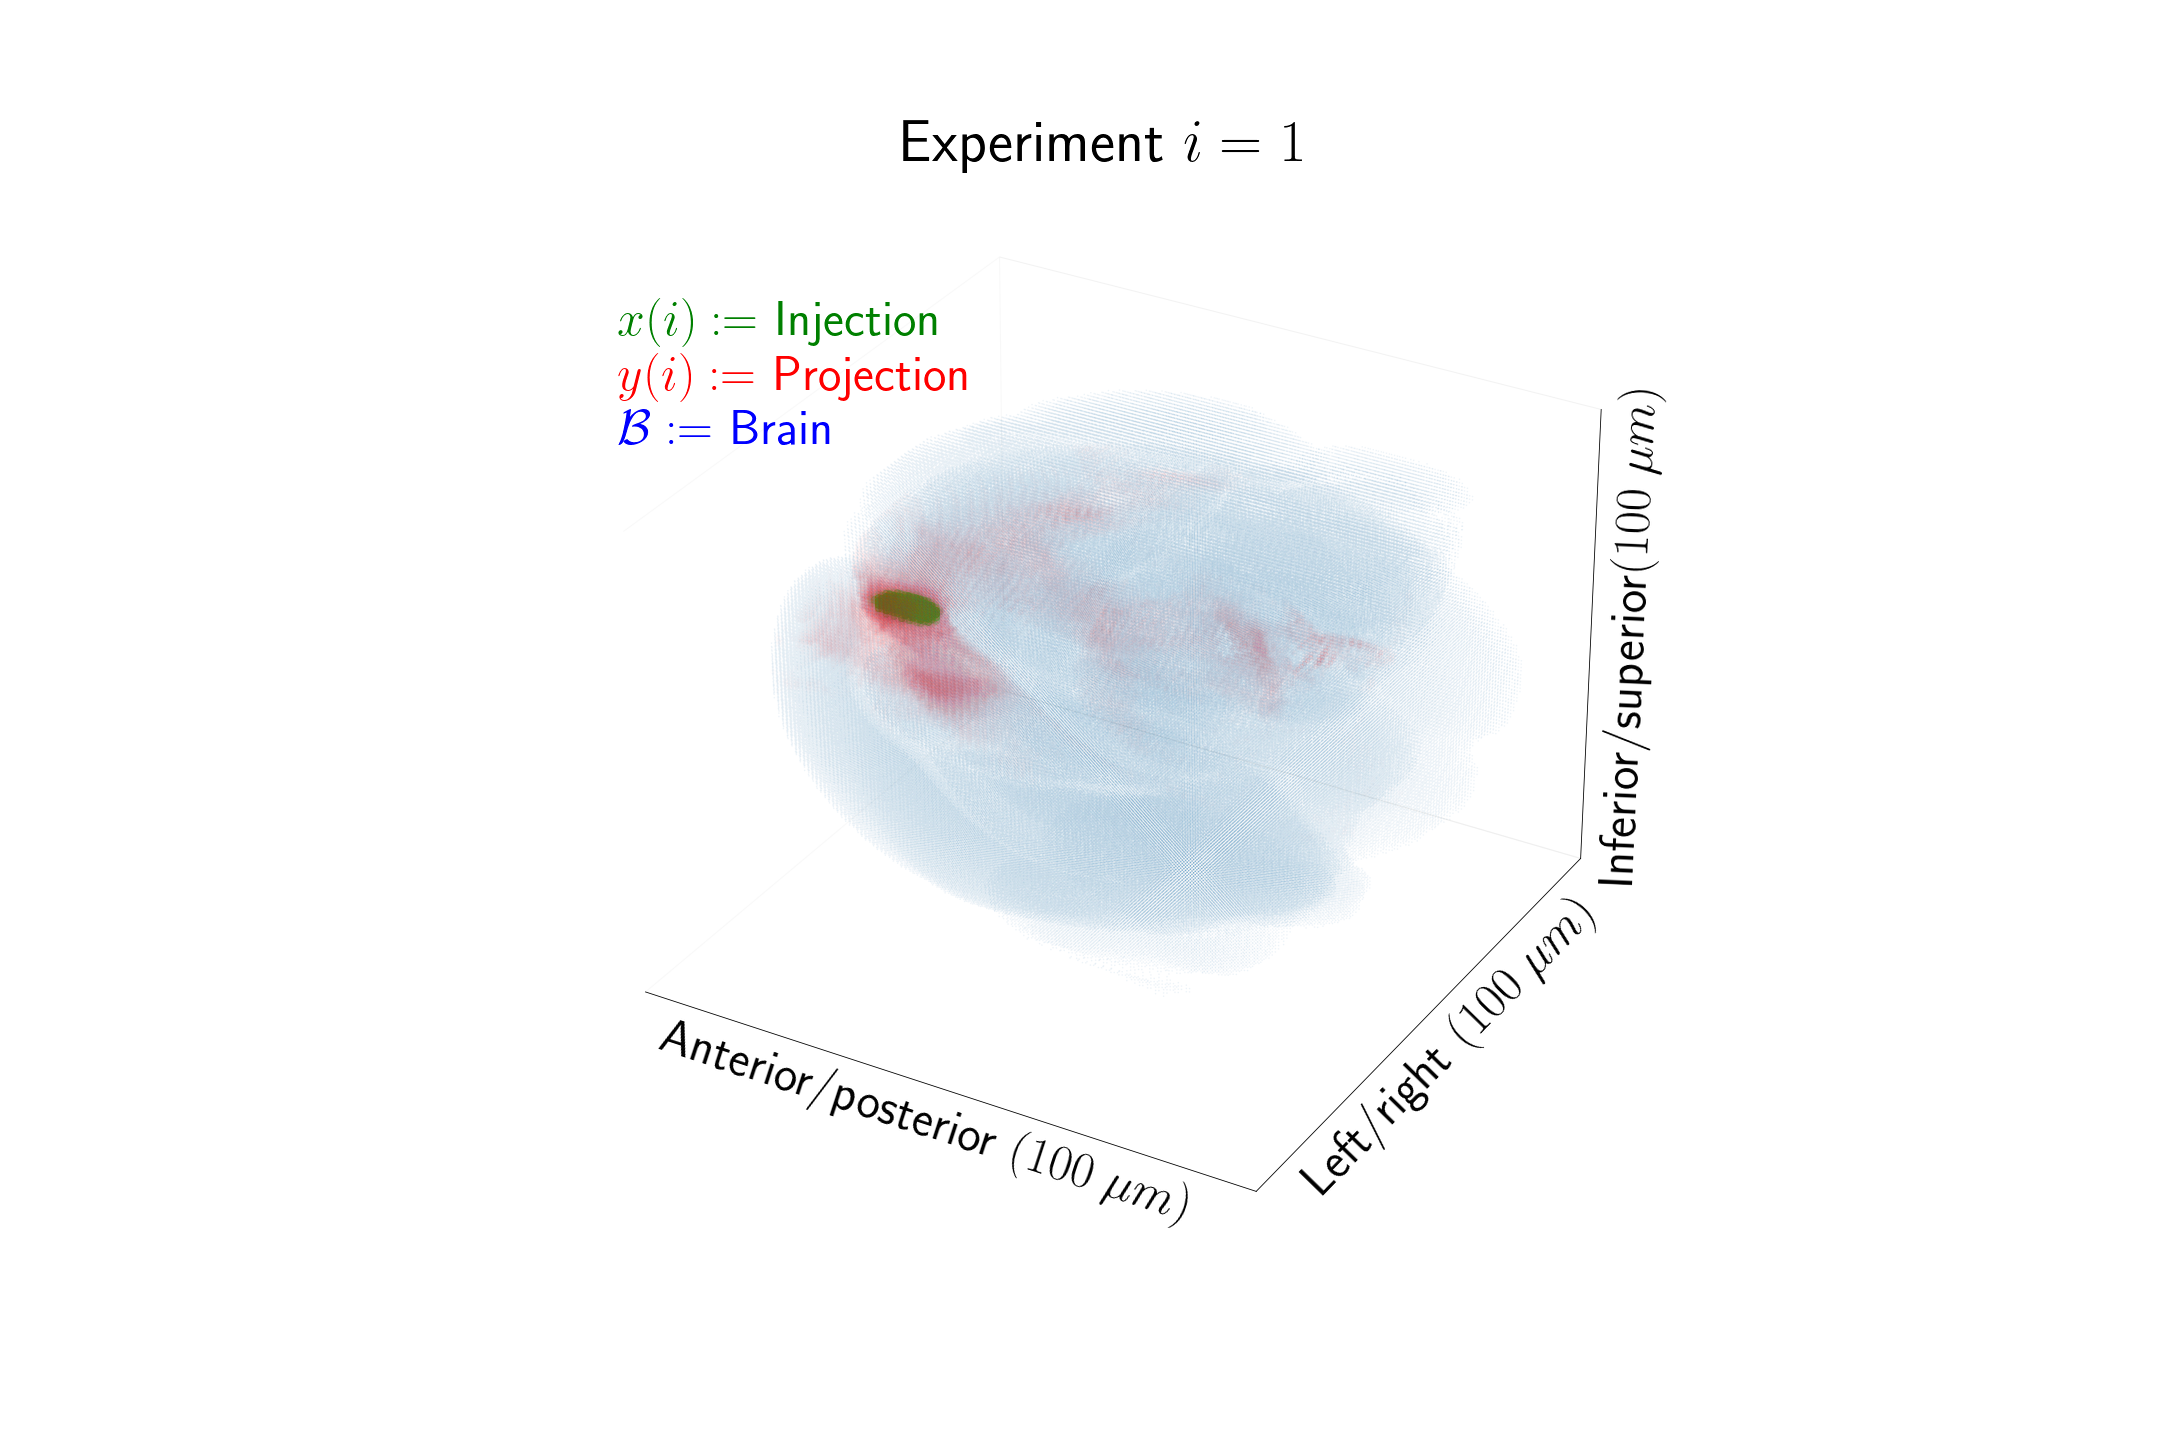
\includegraphics[width=0.4\textwidth]{figs/inj_proj_figure_v2.png}}
\subfloat[]{
    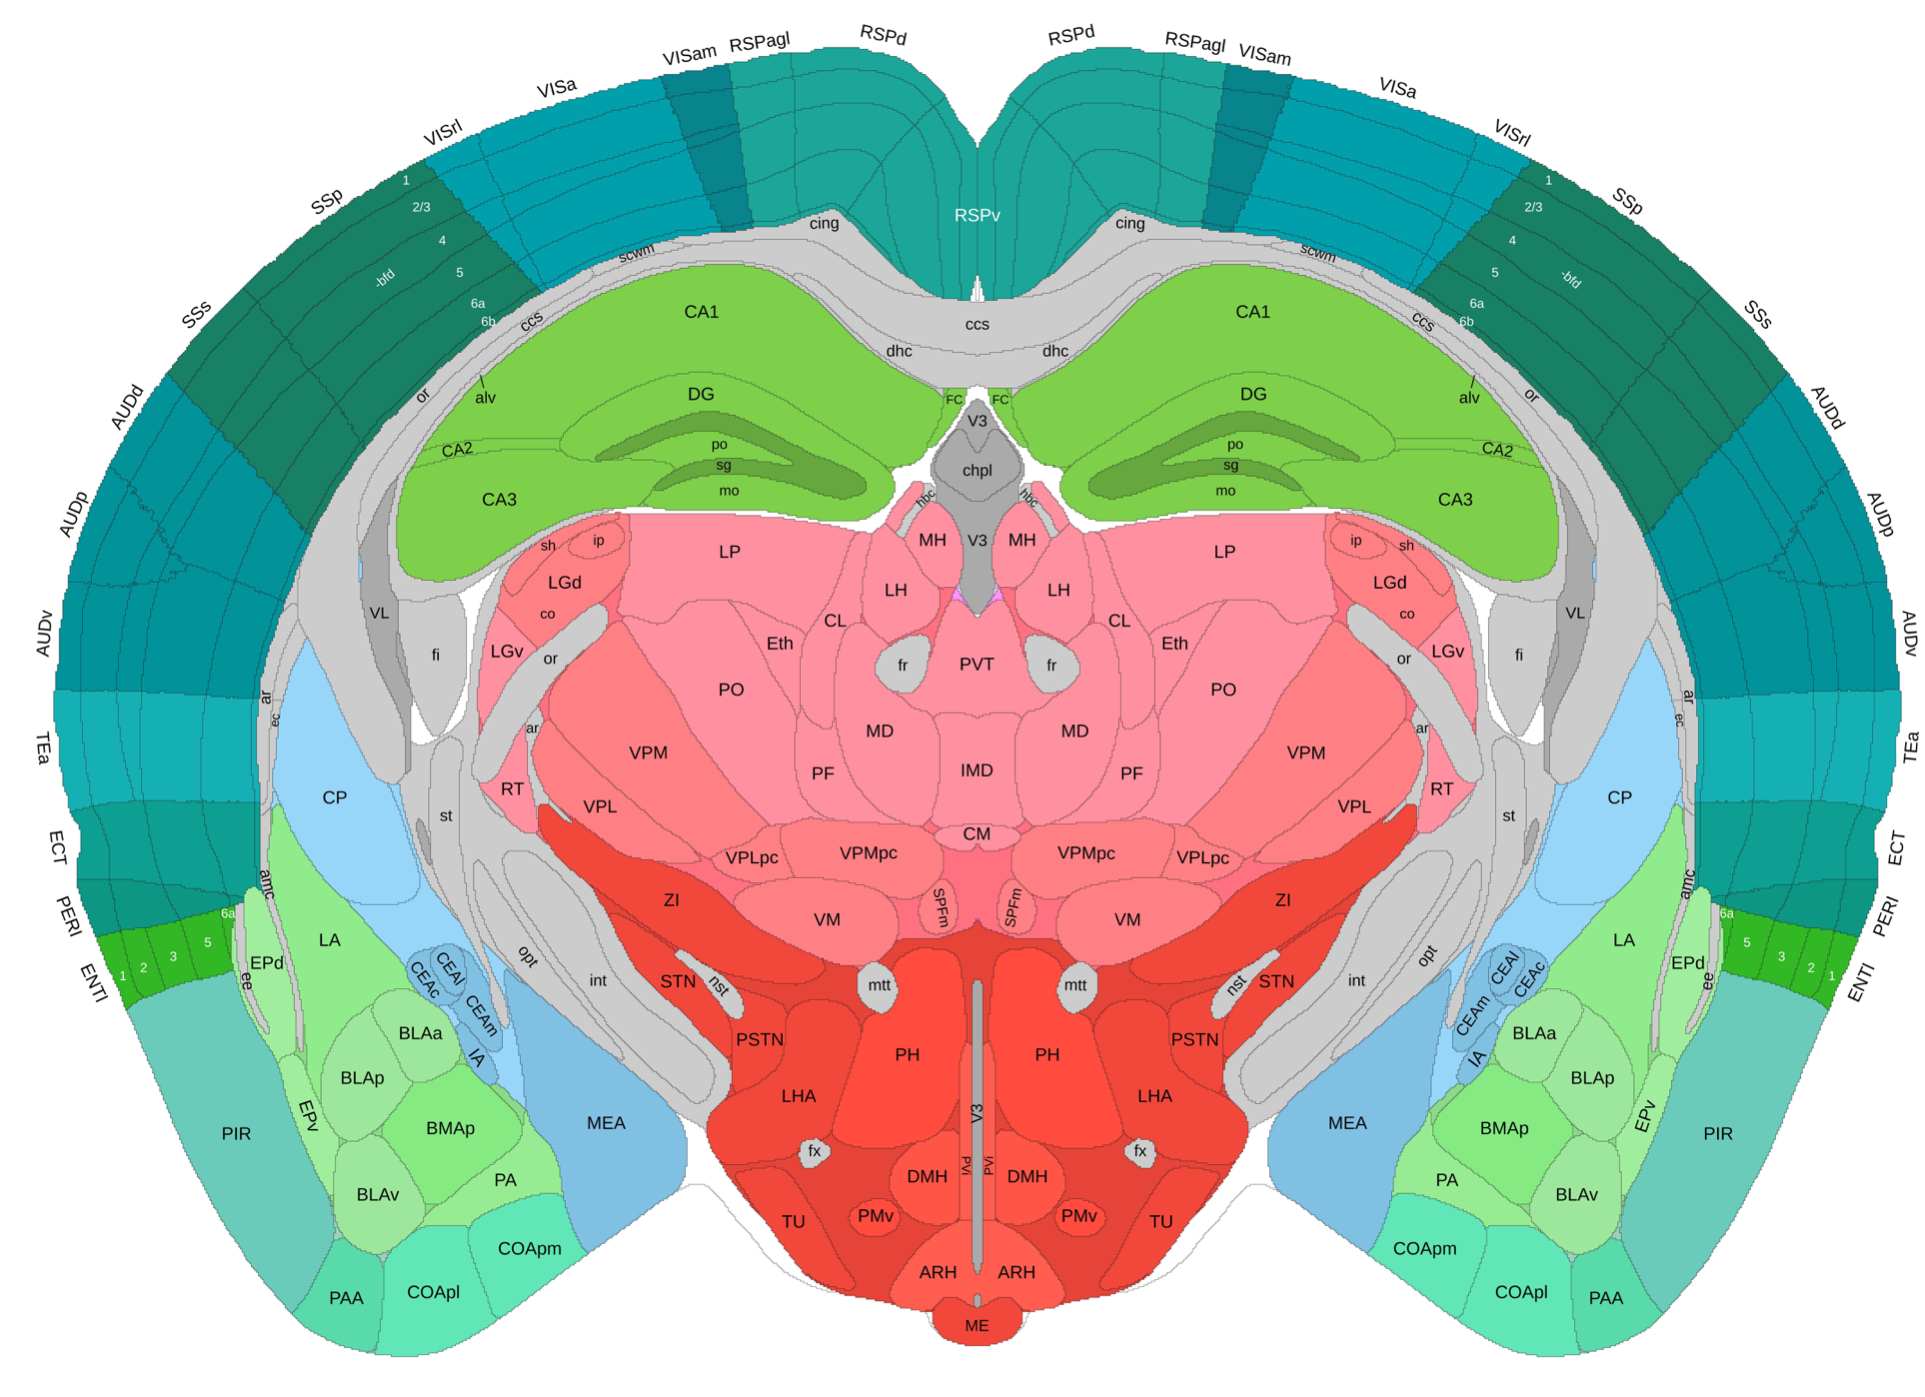
\includegraphics[width=0.3\textwidth]{figs/fig1c.png}}
    \newline
 \subfloat[]{
    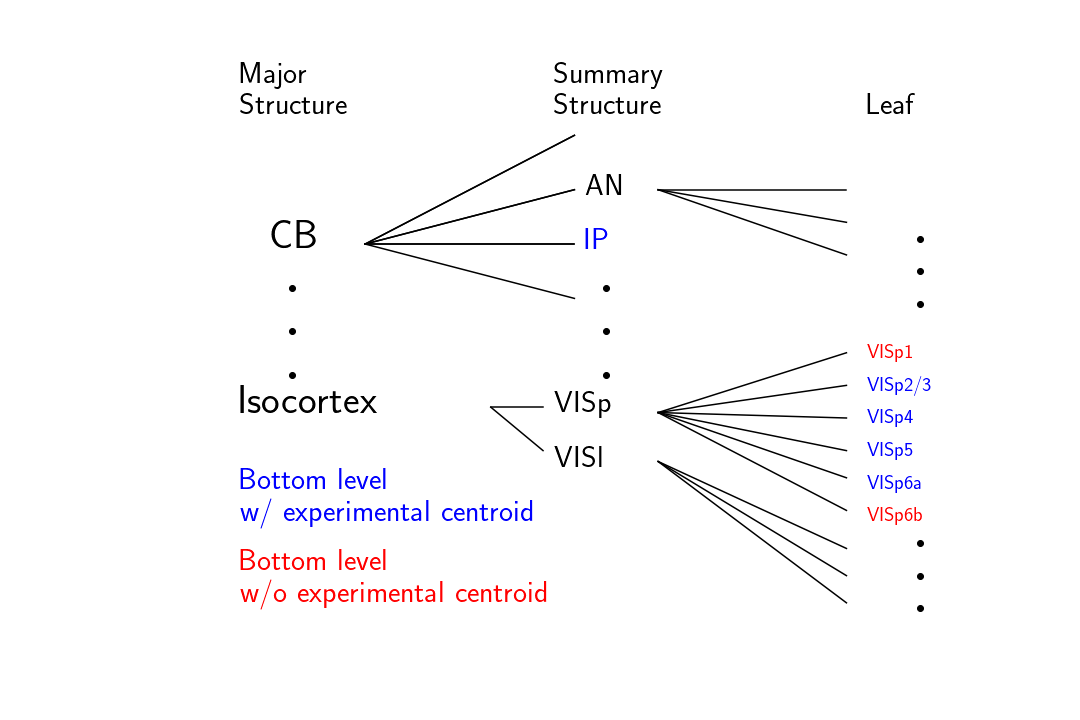
\includegraphics[width=0.35\textwidth]{figs/figsforpres/ontologyfigure.png}}
\subfloat[]{
    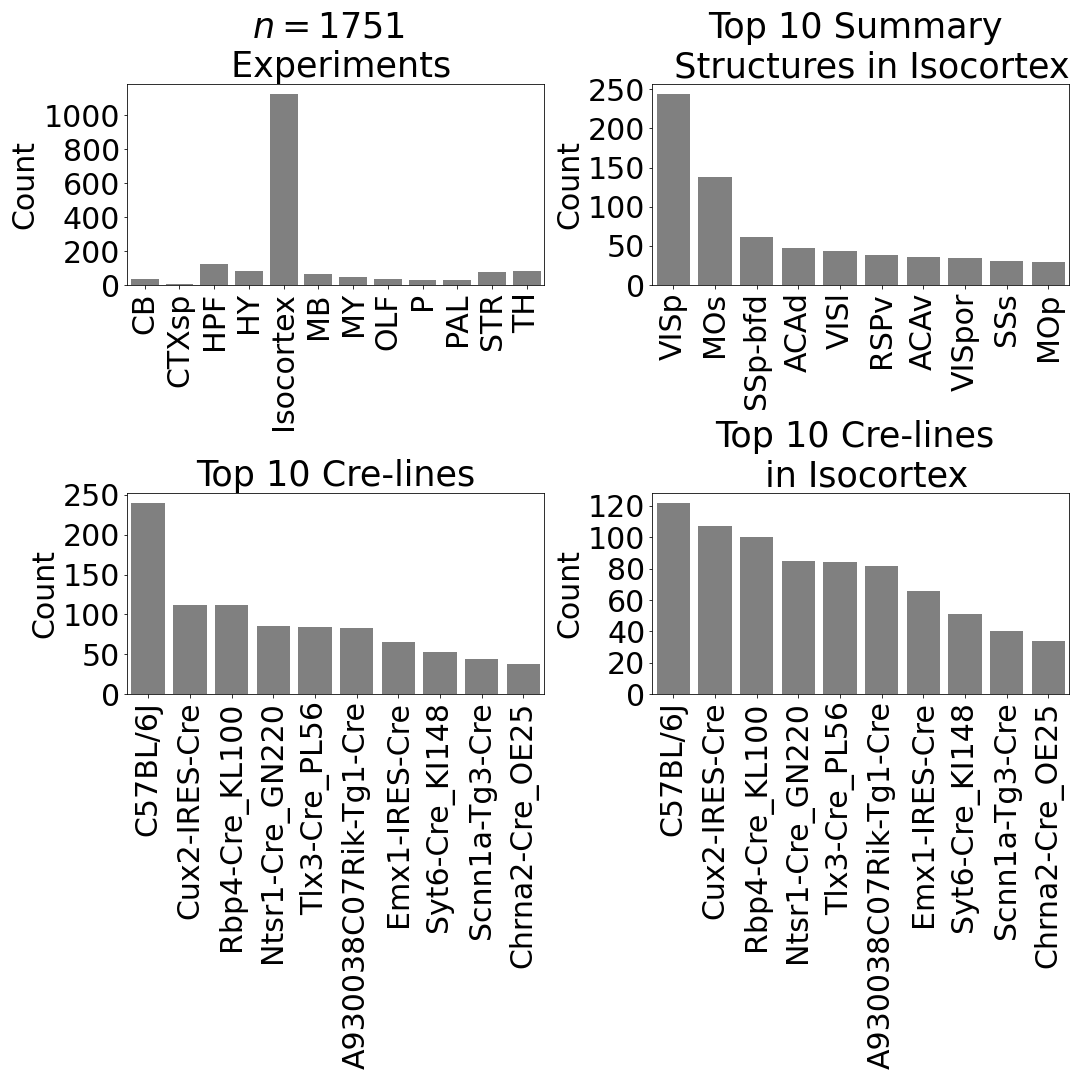
\includegraphics[width=0.35\textwidth]{figs/figsforpres/datasummary.png}}
\subfloat[]{
    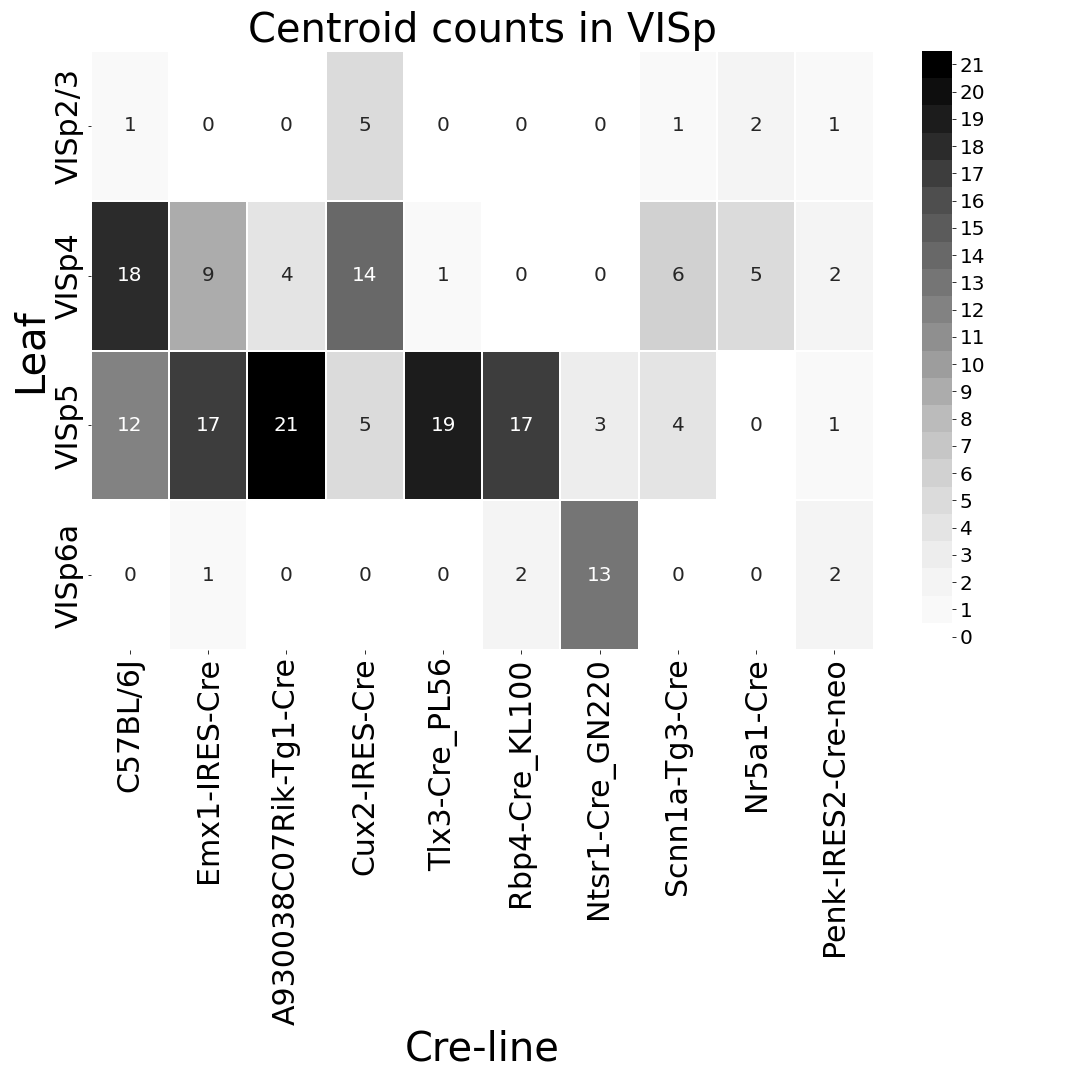
\includegraphics[width=0.35\textwidth]{figs/figsforpres/visp_counts.png}}   
    \caption{a) Background on histology. a) Within the brain (blue), injection (green) and projection (red) areas are determined via histological analysis and alignment to the Allen Common Coordinate Framework (CCF). b) An example of the segmentation of projection and injection for a single experiment. \label{fig:1b} c) Example of structural segmentation within a horizontal plane. d) Explanation of nested structural ontology highlighting lowest-level and data-relevant structures. e) Abundances of crelines and structural injections. f) Co-occurence of layer-specific centroids and creline within VISp}
    \label{fig:data}
\end{figure}
\newpage

%\begin{figure}[H]
 %   \centering
 %   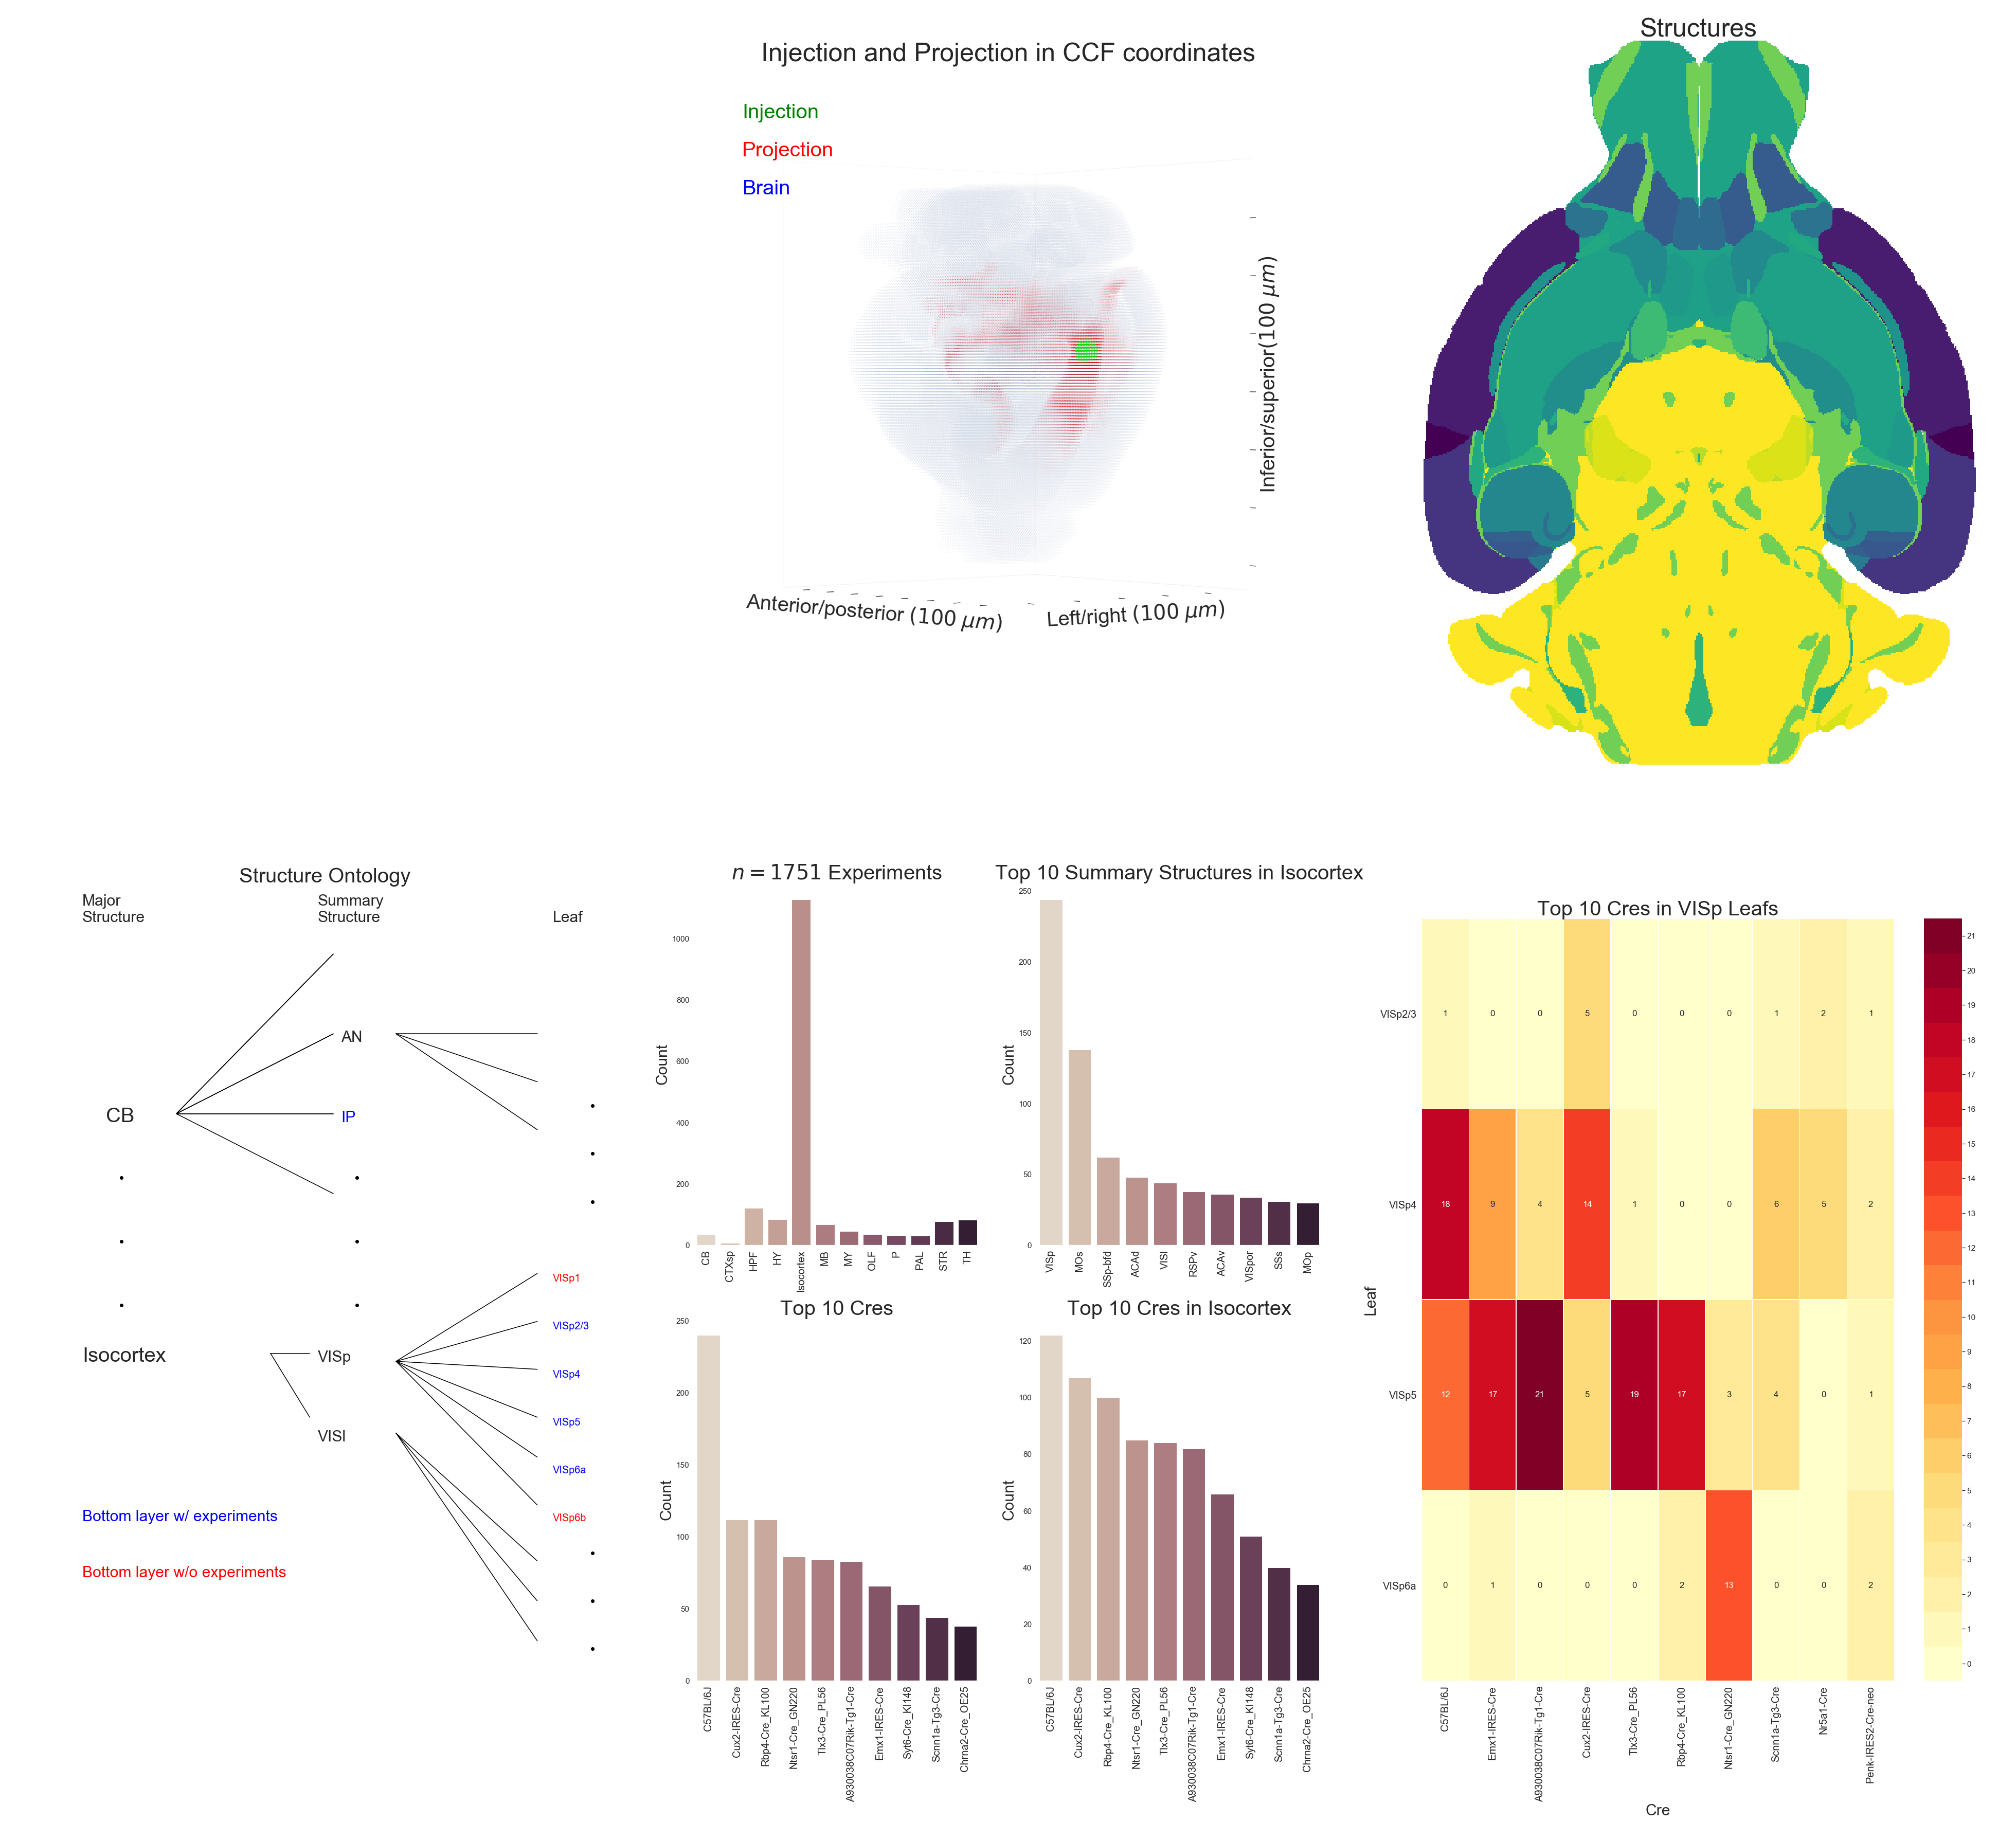
\includegraphics[width = 7in]{figs/figure1draft.png}
%    \caption{a) Background on histology. a) Within the brain (blue), injection (green) and projection (red) areas are determined via histological analysis and alignment to the Allen Common Coordinate Framework (CCF). b) An example of the segmentation of projection and injection for a single experiment. \label{fig:1b} c) Example of structural segmentation within a horizontal plane. d) Explanation of nested structural ontology highlighting lowest-level and data-relevant structures. e) Abundances of crelines and structural injections. f) Co-occurence of layer-specific centroids and creline within VISp}
%    \label{fig:data}
%\end{figure}
%\newpage

Our main result is the creation of cell-type specific connectivity matrices using a model trained on murine viral-tracing experiments.
This section first describes the data used to generate the model, the model itself, evaluation of the model, and the use of the model in creation of the connectivity matrices.
The model we ultimately propose is selected based off it's preferable performance in creation of connectivity matrices with greater accuracy than alternative approaches.
We accompany these matrices with exploratory analyses of the resulting connectivities that illustrate their key features. 

\subsection{Mice}

\skcomment{Experiments involving mice were approved by the Institutional Animal Care and Use Committees of the Allen Institute for Brain Science in accordance with NIH guidelines.}

\subsection{Data}

Our dataset $\mathcal D$ consists of $n=1751$ experiments from the Allen Mouse Brain Connectivity Atlas.
Figure \ref{fig:data} describes the key features of the dataset.
Each experiment is performed by injecting a GFP-labelled transgene casette with a potentially cre-specific promoter into a particular location in a cre-driver mouse.
%Each experiment consists of the injection of a transgene \textit{cre} label into a region of the brain.
The resultant flourescent signal is imaged, and aligned into the Allen Common Coordinate Framework (CCF), a three-dimensional idealized model of the brain that is consistent between animals.

Within the dataset generating the connectivity model reported in this paper, certain structure and cre-line combinations $(S,V)$ appear frequently, while others appear not at all.
Since users of the connectivity matrices may be interested in particular combinations, or interested in the amount of data used to generate a particular connectivity estimate, we exhaustively present this information about all experiments in Appendix \ref*{supp_sec:data}.

\subsection{Data processing}
\label{sec:data_pre}

%In each experiment $i$, injection $x_i \in \mathbb R^{N_i}$ has intensity given by the signal in the $N_i$ voxels in the injection region.
We discretize the fluourescent intensity photographically determined through histological image analysis  at the $100 \; \mu$m \textit{voxel} level.
Thus, the fluorescence is represented as a tensor $\mathcal F \in  \mathbb R^B$ where $B \subset [1:132] \times [1:80] \times [1:104]$ corresponds to the subset of the voxelized $(1.32 \times 0.8 \times 1.04)$ cm rectangular space occupied by the standard mouse brain.
This fluorescence is segmented into \textit{injection} and \textit{projection} areas corresponding to areas of transduction and transduction/transfection, respectively.
For a given experiment, we denote these as $x(i)$ and $y(i)$, respectively.
An example of such segmentation areas is given in Figure \ref{}.
In order to relate the regularly discretized $3D$ space $B$ with biologically informative structures such as the cortex, we also apply several levels of  \textit{regionalization}, as shown in Figure \ref{fig:data}.
Mathematically, we refer to the regionalization map as $r: \mathcal B \times \mathbb R \to \mathcal R \times \mathbb R$.
Given a vector $a$, we also define a normalization map $n: a \mapsto \frac{a}{\sum_{t \in T} a_t}$
A detailed mathematical description of these data preprocessing steps is given in Appendix \ref{sec:dp}.


%Depending on the type of virus, the particular cell-type targeted may vary.  This may effect the observed region.



% Allen CCF space at the $100 \mu m$ {\textit voxel} level, but note that a $10 \mu m$ discretization is also possible \citep{Knox2019-ot}.

%This structural connectivity matrix is the regionalized version of the {\textit local connectivity tensor} $\mathcal C^X \in \mathbb R^{V \times 3 \times 3}$ representing t
%
%Given a set of source regions $S$, target regions $T$, and cre-lines $V$ our goal is the creation of {\textit structural connectivity tensor} $\mathcal C \in \mathbb R^{V \times S \times T}$ representing the strength of the  connection from each source to each target region associated with each cre-line.


%We define the normalized {\textit connection density} $\mathcal C^D$ representing the average connection of a voxel in region $\mathcal S(s)$ to region  $\mathcal T (t)$, and the strength

%and {\textit connection strength} $\mathcal C^S$ 

\subsection{Connectivity}

Our goal is the estimation of {\textit structural connectivity} from one structure to another.
However, at an essential level, cell-class specific neural connectivity is representable as a function $f:  \mathcal V \times \mathbb R^3 \times \mathbb R^3 \to \mathbb R^+$ giving the connection of a particular cell-class from a source position to a target position.
As mentioned in the previous section, our injection and projection intensities are discretized into $100 \mu m$ cubic {\textit voxels}. % \footnote{10 \mu m$ discretization is also possible \citep{Knox2019-ot}}
%These voxels are contained within structures as depicted in Figure \ref{}.
These voxels are contained within structures, so mathematically we can write a region $R= \{r \}$.
We generically denote source regions $S = \{s\}$ and target regions $T = \{t\}$.
%Thus, it is natural to ask what is the 

There are several notions of structural connectivity worth considering based on normalization with respect to the sizes of the source and/or target regions.
Given a set of source regions $\mathcal S = \{ S\} $, target regions $\mathcal T = \{ T \}$, and cre-lines $\mathcal V$ we shall estimate the following tensors:
\begin{align*}
&\text{\textit {connectivity strength} } \mathcal C \in \mathcal V \times \mathcal S \times \mathcal T \times \mathbb R_{\geq 0}  \text{ with } \mathcal C(V,S,T) = \sum_{s \in S} \sum_{t \in  T} f(v,s,t) \\
&\text{\textit {normalized connectivity strength} } \mathcal C^S \in \mathcal V \times \mathcal S \times \mathcal T \times \mathbb R_{\geq 0}  \text{ with } \mathcal C^S(V,S,T) = \frac{1}{|S|} \sum_{s \in  S} \sum_{t \in  T} f(v,s,t) \\
&\text{\textit {normalized projection density} } \mathcal C^D \in \mathcal V \times \mathcal S \times \mathcal T \times \mathbb R_{\geq 0} \text{ with } \mathcal C^D(V,S,T) = \frac{1}{| S | | T|} \sum_{s \in S} \sum_{t \in T} f(v,s,t).
\end{align*}
% \mathbb R^{|\mathcal V| \times |\mathcal S| \times |\mathcal T|} 
Our goal is to estimate $\mathcal C (V,S,T)$ with data $\mathcal D$.
We call this estimator $\widehat { \mathcal C } $.

\subsection{Modelling connectivity}

Construction of such an estimator raises the important questions of 1) what data to use for estimating which connectivity, 2) how to featurize the dataset, 3) what statistical estimator to use, and 4) how to reconstruct the connectivity using the chosen estimator.
Mathematically, we represent these considerations as 
\begin{align}
\label{eq:estimator}
\widehat { \mathcal C }(V,S,T) = e^* (\widehat e (e_*(\mathcal{I} (\mathcal D)))).
\end{align}
This makes explicit the data featurization $e_{*}$, statistical estimator $\widehat e$, and any potential subsequent transformation $e^*$ such as averaging over the source region, as well as the fact that different data $\mathcal D$ may be used to estimate different connectivities.
For example, a simple model would be to take the mean regionalized projection of all the experiments with injection centroid in a given structure.
%The models in \citet{Knox2019-ot} and \citet{Oh2014-kh} use all data from the same major brain division to generate a connectivity for a given structure.
%Note that $\hat f = \widehat e (e_*(\mathcal D))$.
%These questions are intrinsically related, but we separate them for clarity.
Table \ref{tab:estimators} reviews estimators used for this data-type, and explain the intuition behind our new cell-class specific estimator.
Additional information is given in Appendix \ref{supp_sec:el} 
%We also highlight that other combinations 

%The first modelling question is how to featurize the dataset consisting of voxel-level information to best provide structural connectivities.
%The second modelling question is what data to use to estimate each connectivity.
\begin{table}[H]
    \centering
    \begin{tabular}{c|c|c|c|c|}
        Model & $e^*$ & $\widehat e$&  $ e_*$ & Training Data \\
        \hline
        %Leaf-mean & & & & \\
         \citep{Oh2014-kh} & $\widehat e (S)$ & NNLS(X,Y) & $X= r(x(I)),Y = r(y(I))$ & $I = I_M$ \\
        \citep{Knox2019-ot} &$ \sum_{s \in S} \widehat e (s)$ & NW(X,Y)  & $X= c(x(I)), Y = r(y(I))$ & $I = I_M$ \\
        %Cre-leaf-mean & & & & \\
        Cre-NW& $\sum_{s \in S} \widehat e(s)$ & NW(X,Y) & $X= c(x(I)), Y = n(r(y(I)))$  &$I = I_S \cap I_V$ \\
        Expected-loss & $\sum_{s \in S} \widehat e(s)$ & $\text{EL}_S(X,Y,V)$ & $X= c(x(I)), Y = n(r(y(I))), V = v(I)$  &$I = I_S$
    \end{tabular}
    \caption{Estimation of $\mathcal C$ using connectivity data. The regionalization, estimation, and featurization steps are denoted by $e^*, \widehat e,$ and  $e_*$, respectively.
    The training data used to fit the model is given by $I$. We generically denote the set of experiments used to train a particular model as $I$, and experiments from particular major brain divisions, summary structures, and leafs as $I_M$, $I_U$, and $I_L$, respectively.}
    \label{tab:estimators}
\end{table}

Our new methodological contributions in this area - the Cre-NW and Expected-loss models - have several differences from the previous methods.
Both the \citet{Oh2014-kh} non-negative least squares and \citet{Knox2019-ot} Nadaraya-Watson take into account $s$ and $t$, but not $v$.
Since our goal is creation of cre-specific connectivities, our new estimators specifically account for this information.
The cre-specific Nadaraya-Watson estimator only uses experiments from a particular cre-line to predict cell-class connectivity, while the Lxpected Loss estimator shares information between cre-lines.
We also normalize projections by total intensity to account for differences in the cre-driven expression of eGFP via the various transgene promoters.

%The third modelling question is what classes of estimators $\hat f$ to consider.
%We evaluate several different candidate estimators.
%The first is the non-negative least squares estimator that was applied to connectivity data in \citet{Oh2014-kh}, and the second is the Nadaraya-Watson estimator that was applied to connectivity data in \citet{Knox2019-ot}.

%Both of these estimators perform better than the estimator in \citet{Knox2019-ot} across the whole dataset, and comparably well in wild-type, while the Expected Loss estimator in general gives the best performance.

The final and perhaps most important modelling question is how to select optimum functions from within and between these estimator classes.
Examining Equation \ref{eq:estimator}, we can see that in $3D$ coordinates, $\widehat f(v,s,t) = \widehat e (e_*(\mathcal{I} (\mathcal D)))$, with $e^*$ a deterministic step that is determined without input by the data.
Thus, we can evaluate our model by it's ability to predict held-out experiments in {\textit leave-one-out cross validation}.
%Thus, when comparing models specific to larger or smaller subsets (e.g. a model based off of all experiments in a leaf with a model based off of all wild-type experiments in a leaf), we should evaluate both on the experiments suggested by the smaller set.
In order to compare between methods, we necessarily restrict to the smallest set of evaluation experiments suggested by any of our models - that is, those with combinations of cre-line and structure-leaf that are present at least twice.
We use $l2$-loss and weighted $l2$-loss to evaluate these predictions:
\begin{align*}
\text{l2-loss } l ( \hat f) &= \frac{1}{|I_M|} \sum_{i \in I_M} \| r(y(i)) - \hat f(c(i)) \|_2^2 \\
\text{weighted l2-loss } l ( \hat f) &= \frac{1}{|\{S,V\}|} \sum_{s,v \in \{S,V\}} \frac{1}{ |I_{s,v}|} \sum_{i \in I_{s,v} } l(r(y(i)), \hat f(\mathbb D \setminus i)) 
\end{align*}
Due to our normalizing preprocessing step, the former is equivalent to the normalized loss in \citet{Knox2019-ot}, and also to cosine loss, while the latter weights all region cell-class combinations equally.

As a final modelling step, we establish a lower limit of detection.
This is covered in Appendix.
%The subsequent subsections describe our estimators and our model evaluation criteria, while Section \ref{sec:model_eval} gives details on model performance.

%Since our models incorporate cre-lines and structure information in a diverse set of ways, our evaluation set is constructed in order to be shareable between all models.
%This method robustly handles overfitting in Nadaraya-Watson bandwidth selection.

%to say, cre-leaf combinations that are present at least twice. 
%The most restrictive evaluation set is, in general, suggested by the class of models with training data given by a specific combination of cre-line and leaf.
%We therefore evaluate all models on this set.
%We also remove points from their own target-encoded mean in the expected-loss estimator, alghough instances, for the same type of point, should be zero.

\subsection{Connectivity analyses}

%Many interesting neuronal processes underly our estimated connectome. 
%We quantify several of these through posthoc analyses.
We quantify and illustrate some of the interesting neuronal processes underlying our estimated connectome.
First, we cluster projection pattern by cell-class and source structure.
This shows that cell-class has a dominating effect on projection in certain regions.
Second, we extend the characterization of \citet{Knox2019-ot} on structural differences in short-range projections.
These are primarily assumed to be due to diffusion, and the diffusion-rate helps to characterize the basic structural anatomy.
Third, since the overall wild-type connectome results from the combination of underlying cell-classes, we apply non-negative matrix factorization (NMF) to decompose the observed long-range connectivity into \textit{connectivity archetypes} that linearly combine to reproduce the observed connectivity.
These methods identify structures with both known and plausible biological meaning, and simplistically exemplify useful posthoc analyses for data of this type.
Technical details of these approaches are given in Appendix.
%types of latent structure in the estimated connectivities.
%As a simple proof of the cell-class specific nature of $\mathcal C$, we cluster regional projections estimated for combinations of structure and cell-class.

%Under this hypothesis, unsupervised learning algorithms provide useful reduced-dimensional descriptions of the data-generating mechanism.
%We therefore apply heirarchical clustering to illustrate which source and cell-type combinations behave similarly, and non-negative matrix factorization to estimate a dimensionality of the latent space of biological processes, as well which target projections tend to co-occur.


%\paragraph{Factoring the connectivity tensor with heirarchical clustering}

%Heirarchical clustering is an algorithm for uncovering similar data points available in many computational libraries.
%We flatten the connectivity tensor $\mathcal C \in \mathbb R^{c \times s \times t}$ to $\mathcal C_\flat \in \mathbb R^{c s \times t}$ and cluster the $cs$ sources by their $t$-dimensional projections.
%Clustered source-cell combinations have similar projection patterns.

%In particular, we illustrate which source and cell-type combinations behave similarly, and which target projections tend to co-occur. 

%\paragraph{Factoring cell-type specific tensors with censored NMF}

%Non-negative matrix factorization refers to a collection of dictionary-learning algorithms for decomposing a positively-valued matrix such as $\mathcal C $ into positively-valued matrices called, by convention, weights $W \in \mathbb R^{| \mathcal {S}| \times s}_{\geq 0}$ and hidden units $H \in \mathbb R^{l  \times | \mathcal {T}|}_{\geq 0}$.
%Like PCA, NMF identifies a low dimensional latent space.
%In contrast to PCA, the $l$ components of $\hat H$ are not necessarily orthogonal, and the objective is generally not unique.

%Since the large short-range projections resulting from diffusion dominate the matrices $\hat {\mathcal C}$, we ignore connections between source and and target regions less than $1500 \mu m$ apart.
%We use unsupervised cross-validation to determine $l$.
%We also account for the difficult-to-optimize NMF optimization problem by running multiple replicates, and clustering the resulting $H$.
%We use stability to determine a superset of clusters, and select the median-vectors of the $l$ most common clusters as connectivity \textit{ archetypes}.
%The latter issue is ameliorated by regularization terms to encourage finding vectors around which  $\hat {\mathcal C}$ is clustered.
%

%As in \citet{Knox2019-ot}, we divide the brain into 12 {\it major brain divisions} $M$ (the isocortex, olfactory areas, hippocampal formation, cortical subplate, striatum, pallidum, thalamus, hypothalamus, midbrain, pons, medulla, and cerebellum), and, at a finer level, divide the brain into 286 ipsilateral, 5 medial, and 286 contralateral summary structures {\it summary structures} $R$.

%We also introduce an even finer, leaf-specific, decomposition $L$, with $|L| = 1077$.

%In contrast to \citet{Knox2019-ot}, which only uses wild type $C57BL/6J$ mice, these experiments utilize $113$ different transgene cassettes. 

%In these coordinates, the brain $B \subset \mathbb R^{131 \times 75 \times 108)}$ is discretized into 100-$\mu m$ wide cubes known as voxel. This is shown in Figure \ref{fig:data_process}.

%$B \subset \mathbb R^{a \times b \times c}$, where the coordinate discretezation of $B$ is at the 100 micrometer resolution.
% The injection and projection signals $x(1:n) \in B$ and $y(1:n) \in B$ respectively are determined via histology. Note that the histologically determined injection and projection regions may subsegment individual voxels. Therefore, the injection is determined by element-wise multiplication of the injection and projection with the fraction contained in the injection region. 
%Check if injection is just masked projection in allen_sdk download (i.e. at first step)

%Injections and projections were downloaded using the Allen SDK. These were originally annotated manually. The injection and projection vectors are adjusted by a data quality matrix.

\section{Results}

Our results include evaluation of model fit, the cre-specific connectivity matrices themselves, and retrospective analyses of these matrices for  patterns related to cre-type and source and target regions.

\subsection{Model evaluation}
\label{sec:model_eval}

%Note that this is also the largest evaluation set for 2-stage model, since leave-one-out means of each cre-line may only be computed for lines which are present at least twice in the leaf.
Table  contains the sizes of these evaluation sets in each major structure.
This information may be cross-referenced visually with the figures in 
Our two-stage model generally performs better than the cre-line specific NW estimator.


\newpage 
\begin{table}[H]
\begin{adjustbox}{width=.5\columnwidth,center}

\begin{tabular}{ll|rrrrr}
\toprule
   & Estimator &     EL &     NW & Average &     NW &  NW-wt \\
   & Smoothing &     SS & Cre-SS &  Cre-SS &     SS &      M \\
   & Target &     SS &     SS &      SS &     SS &     SS \\
Structure & \# Eval exps &        &        &         &        &        \\
\midrule
\hline
CB & 10 &  0.044 &  0.081 &   0.081 &  0.058 &  0.439 \\
CTXsp & 2 &  0.497 &  0.497 &   0.497 &  0.497 &  0.000 \\
HPF & 79 &  0.122 &  0.140 &   0.143 &  0.155 &  0.471 \\
HY & 41 &  0.241 &  0.266 &   0.269 &  0.244 &  1.019 \\
Isocortex & 838 &  0.173 &  0.195 &   0.202 &  0.234 &  0.404 \\
MB & 23 &  0.151 &  0.151 &   0.166 &  0.139 &  0.759 \\
MY & 7 &  0.186 &  0.233 &   0.233 &  0.184 &  0.452 \\
OLF & 17 &  0.069 &  0.095 &   0.100 &  0.073 &  0.110 \\
P & 8 &  0.236 &  0.239 &   0.239 &  0.264 &  0.984 \\
PAL & 11 &  0.190 &  0.198 &   0.198 &  0.260 &  1.401 \\
STR & 45 &  0.084 &  0.088 &   0.089 &  0.097 &  0.265 \\
TH & 29 &  0.351 &  0.678 &   0.678 &  0.365 &  1.088 \\
\bottomrule
\end{tabular}
\end{adjustbox}
\caption{Weighted losses with summary structure targets.}
\end{table}

\begin{comment}
\resizebox{1.5in}{!}{%
\begin{tabular}{lr}
\toprule
Estimator &     Expected-loss \\
Smoothing &              Leaf \\
Target & SS \\
\midrule
CB        &             0.042 \\
CTXsp     &             0.497 \\
HPF       &             0.087 \\
HY        &             0.221 \\
Isocortex &             0.125 \\
MB        &             0.120 \\
MY        &             0.155 \\
OLF       &             0.058 \\
P         &             0.229 \\
PAL       &             0.147 \\
STR       &             0.049 \\
TH        &             0.295 \\
\bottomrule
\end{tabular}
}

\begin{tabular}{llr}
\toprule
   & Estimator &     Expected-loss \\
   & Smoothing &              Leaf \\
   & Target & Summary Structure \\
Structure & \# Eval exps &                   \\
\midrule
CB & 4   &             0.042 \\
CTXsp & 2   &             0.497 \\
HPF & 62  &             0.087 \\
HY & 41  &             0.221 \\
Isocortex & 732 &             0.125 \\
MB & 18  &             0.120 \\
MY & 7   &             0.155 \\
OLF & 17  &             0.058 \\
P & 8   &             0.229 \\
PAL & 11  &             0.147 \\
STR & 45  &             0.049 \\
TH & 29  &             0.295 \\
\bottomrule
\end{tabular}


\newpage
\begin{table}[H]
%\small
\begin{tabular}{l|rrrrrr}
\toprule
{} &  \thead{NW w/in \\ SS} &  \thead{NW w/in \\ cre-SS combo} &   \thead{NW w/in \\ leaf} &   \thead{NW w/in \\ cre-leaf combo} &   \thead{2-stage w/in \\ SS} &  \thead{2-stage w/in \\ leaf} \\
\midrule
Isocortex &    0.197949 &              0.140132 &      0.184242 &                0.150736 &         0.123061 &           0.127477 \\
OLF       &    0.063727 &              0.074488 &      0.063727 &                0.074488 &         0.048604 &           0.055660 \\
HPF       &    0.123701 &              0.093232 &      0.112693 &                0.101307 &         0.079024 &           0.083872 \\
CTXsp     &    0.496673 &              0.496673 &      0.496673 &                0.496673 &         0.496673 &           0.496673 \\
STR       &    0.081748 &              0.063708 &      0.081748 &                0.063708 &         0.049181 &           0.048064 \\
PAL       &    0.256060 &              0.194300 &      0.256060 &                0.194300 &         0.119387 &           0.137670 \\
TH        &    0.314873 &              0.572374 &      0.314612 &                0.572254 &         0.283193 &           0.326897 \\
HY        &    0.240828 &              0.259324 &      0.240828 &                0.259324 &         0.203881 &           0.219835 \\
MB        &    0.139129 &              0.119975 &      0.129236 &                0.119420 &         0.108631 &           0.112262 \\
P         &    0.264159 &              0.238584 &      0.264159 &                0.238584 &         0.206783 &           0.228114 \\
MY        &    0.201169 &              0.224394 &      0.201169 &                0.224394 &         0.118224 &           0.163585 \\
CB        &    0.039459 &              0.049516 &      0.039459 &                0.049516 &         0.024929 &           0.038626 \\
\bottomrule
\end{tabular}
\caption{Leave-one-out cross-validation results for experiments at the summary-structure level.}
\end{table}

\newpage

\begin{table}[H]
%\small
\begin{tabular}{l|rrrrrr}
\toprule
{} &  \thead{NW w/in \\ SS} &  \thead{NW w/in \\ cre-SS combo} &   \thead{NW w/in \\ leaf} &   \thead{NW w/in \\ cre-leaf combo} &   \thead{2-stage w/in \\ SS} &  \thead{2-stage w/in \\ leaf} \\
\midrule
Isocortex &    0.308850 &              0.170937 &      0.276799 &                0.183782 &         0.157795 &           0.156463 \\
OLF       &    0.055691 &              0.065967 &      0.055691 &                0.065967 &         0.050010 &           0.045780 \\
HPF       &    0.145990 &              0.100792 &      0.127685 &                0.107282 &         0.092406 &           0.087957 \\
CTXsp     &    0.601404 &              0.601404 &      0.601404 &                0.601404 &         0.601404 &           0.601404 \\
STR       &    0.080912 &              0.060845 &      0.080912 &                0.060845 &         0.045861 &           0.046731 \\
PAL       &    0.239272 &              0.201293 &      0.239272 &                0.201293 &         0.147122 &           0.124190 \\
TH        &    0.308351 &              0.536464 &      0.309573 &                0.537646 &         0.296443 &           0.261895 \\
HY        &    0.243442 &              0.267104 &      0.243442 &                0.267104 &         0.214046 &           0.203092 \\
MB        &    0.217693 &              0.159905 &      0.193525 &                0.158817 &         0.144303 &           0.138584 \\
P         &    0.346317 &              0.250512 &      0.346317 &                0.250512 &         0.257404 &           0.235210 \\
MY        &    0.196393 &              0.222365 &      0.196393 &                0.222365 &         0.161073 &           0.115752 \\
CB        &    0.039327 &              0.049425 &      0.039327 &                0.049425 &         0.038542 &           0.024803 \\
\bottomrule
\end{tabular}
\caption{Leave-one-out cross-validation results for experiments at the leaf level.}
\end{table}
\end{comment}



\newpage

\subsection{Connectivities}

Our main result is the estimation of matrices $\hat {\mathcal C}_v$ representing connections of source structures to target structures for particular cre-lines $v$. 
We exhibit several characteristics of interest, and confirm the detection of several well-established connectivities within our tensor.
Many additional interesting biological processes are visible within this matrix - more than we can report in this paper - and it is our expectation that these will be identified by users of our results.
The connectivity tensor and code to reproduce it are available at \skcomment{footnote}.

The connectivity matrix for wild-type connectivities from leaf sources to summary structure targets is illustrated in Figure \ref{fig:connectome}.
The clear intraareal connectivities mirror previous estimates in \citet{Oh2014-kh} and \citet{Knox2019-ot} and descriptive depictions of individual experiments in \citet{Harris2019-mr}.
Compared with \citet{Knox2019-ot}, our more discritized source smoothing and greater number of experiments leads to a significantly more discritized connectivity matrix.
This is generally expected - for example, different cortical layers have more substantially different connectivities.

The cell-type specific connectivities that we provide also conform to well-known behaviors.
Examples from the visual processing and motor control regions of the cortex are given in Figure \ref{fig:visp_mo_1201} for both wild type and several cre-lines.
Rbp4-Cre and Ntsr1-Cre target layers $5$ and $6$, respectively. As in \citet{Jeong2016-dc}, layer 5 projects to anterior basolateral amygdala (BLA) and capsular central amygdala (CEA), while layer 6 does not.

\newpage

\begin{figure}[h]
\centering
    \subfloat[] {
   % \raisebox{-.5\height}
    \includegraphics[width = \linewidth]{wt_conn_sumleaf_strength.png}
    } 
    \\
    \vspace{-2cm}
    \subfloat[]{
    \adjustbox{valign=c}{
    \tiny
\begin{tabular}{lrllll}
\toprule
{} &  \#\pbox{20cm} {Ipsilateral \\ Leaf Targets } & \pbox{20cm}{Top \\ Entropy }& Bottom Sparsity & Bottom Entropy & Top Sparsity \\
\midrule
Isocortex &                          51 &          CP &             BAC &            BAC &         ENTl \\
OLF       &                          11 &         TMv &             III &            III &          NaN \\
HPF       &                          15 &          IG &             EPv &             PA &          NaN \\
CTXsp     &                           7 &          TT &              FC &            APr &           TT \\
STR       &                          14 &         RPA &             ISN &            PYR &           TU \\
PAL       &                           9 &          PG &           ACVII &             GR &           MG \\
TH        &                          44 &         NOD &              DN &         SSp-ll &          SCm \\
HY        &                          44 &         CLA &              SH &            LSc &           DG \\
MB        &                          39 &         NDB &            SubG &            SGN &          SUB \\
P         &                          26 &          MT &            Acs5 &            SOC &          NDB \\
MY        &                          43 &          RT &             NaN &             OV &          EPd \\
CB        &                          18 &         ECT &             AOB &            MOB &           GU \\
\bottomrule
\end{tabular}
    }
}
    \subfloat[]{
    \adjustbox{valign=c}{
    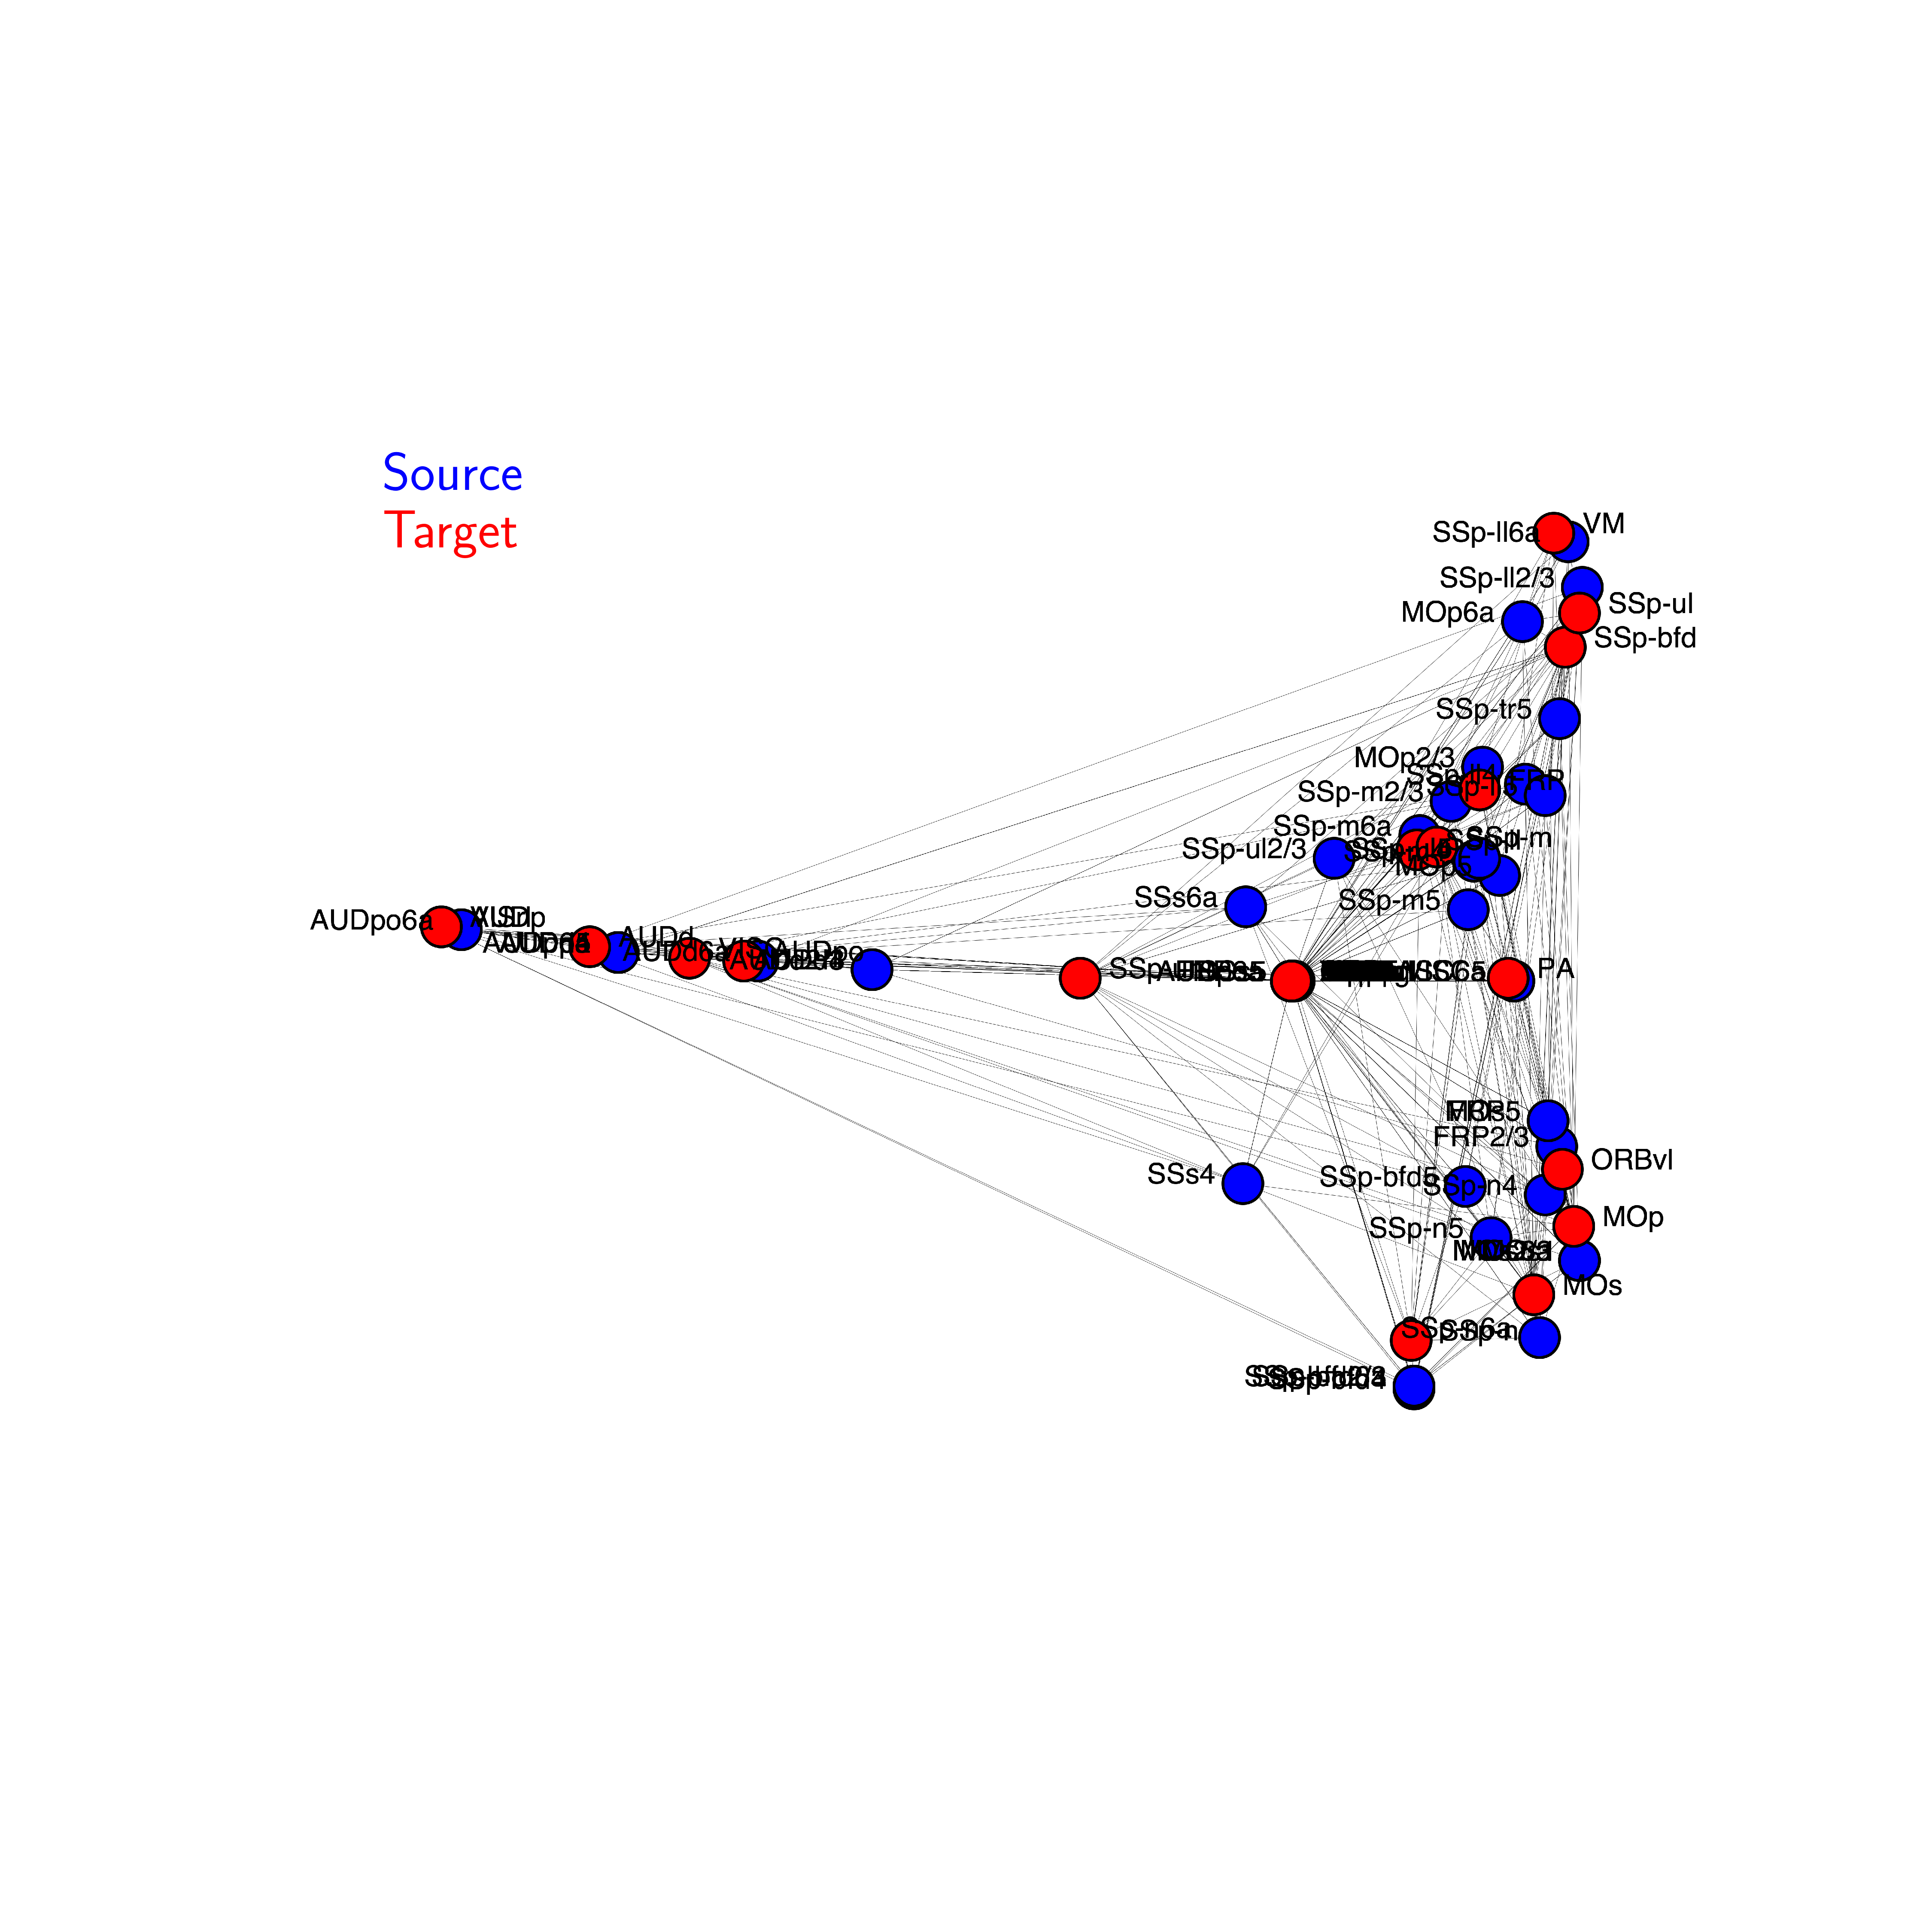
\includegraphics[width = 3in]{figs/st_graph}
    }
    } \\
     \vspace{-4cm}
    \subfloat[]{
    \adjustbox{valign=c}{
    \tiny
    \begin{tabular}{lrllll}
       
\toprule
{} &  \# Ipsilateral Leaf Targets & Top Entropy & Bottom Sparsity & Bottom Entropy & Top Sparsity \\
\midrule
Isocortex &                          51 &          CP &             BAC &            BAC &         ENTl \\
OLF       &                          11 &         TMv &             III &            III &          NaN \\
HPF       &                          15 &          IG &             EPv &             PA &          NaN \\
CTXsp     &                           7 &          TT &              FC &            APr &           TT \\
STR       &                          14 &         RPA &             ISN &            PYR &           TU \\
PAL       &                           9 &          PG &           ACVII &             GR &           MG \\
TH        &                          44 &         NOD &              DN &         SSp-ll &          SCm \\
HY        &                          44 &         CLA &              SH &            LSc &           DG \\
MB        &                          39 &         NDB &            SubG &            SGN &          SUB \\
P         &                          26 &          MT &            Acs5 &            SOC &          NDB \\
MY        &                          43 &          RT &             NaN &             OV &          EPd \\
CB        &                          18 &         ECT &             AOB &            MOB &           GU \\
\bottomrule
\end{tabular}
}
}
\vspace{-4cm}
    \subfloat[]{
    \adjustbox{valign=c}{
    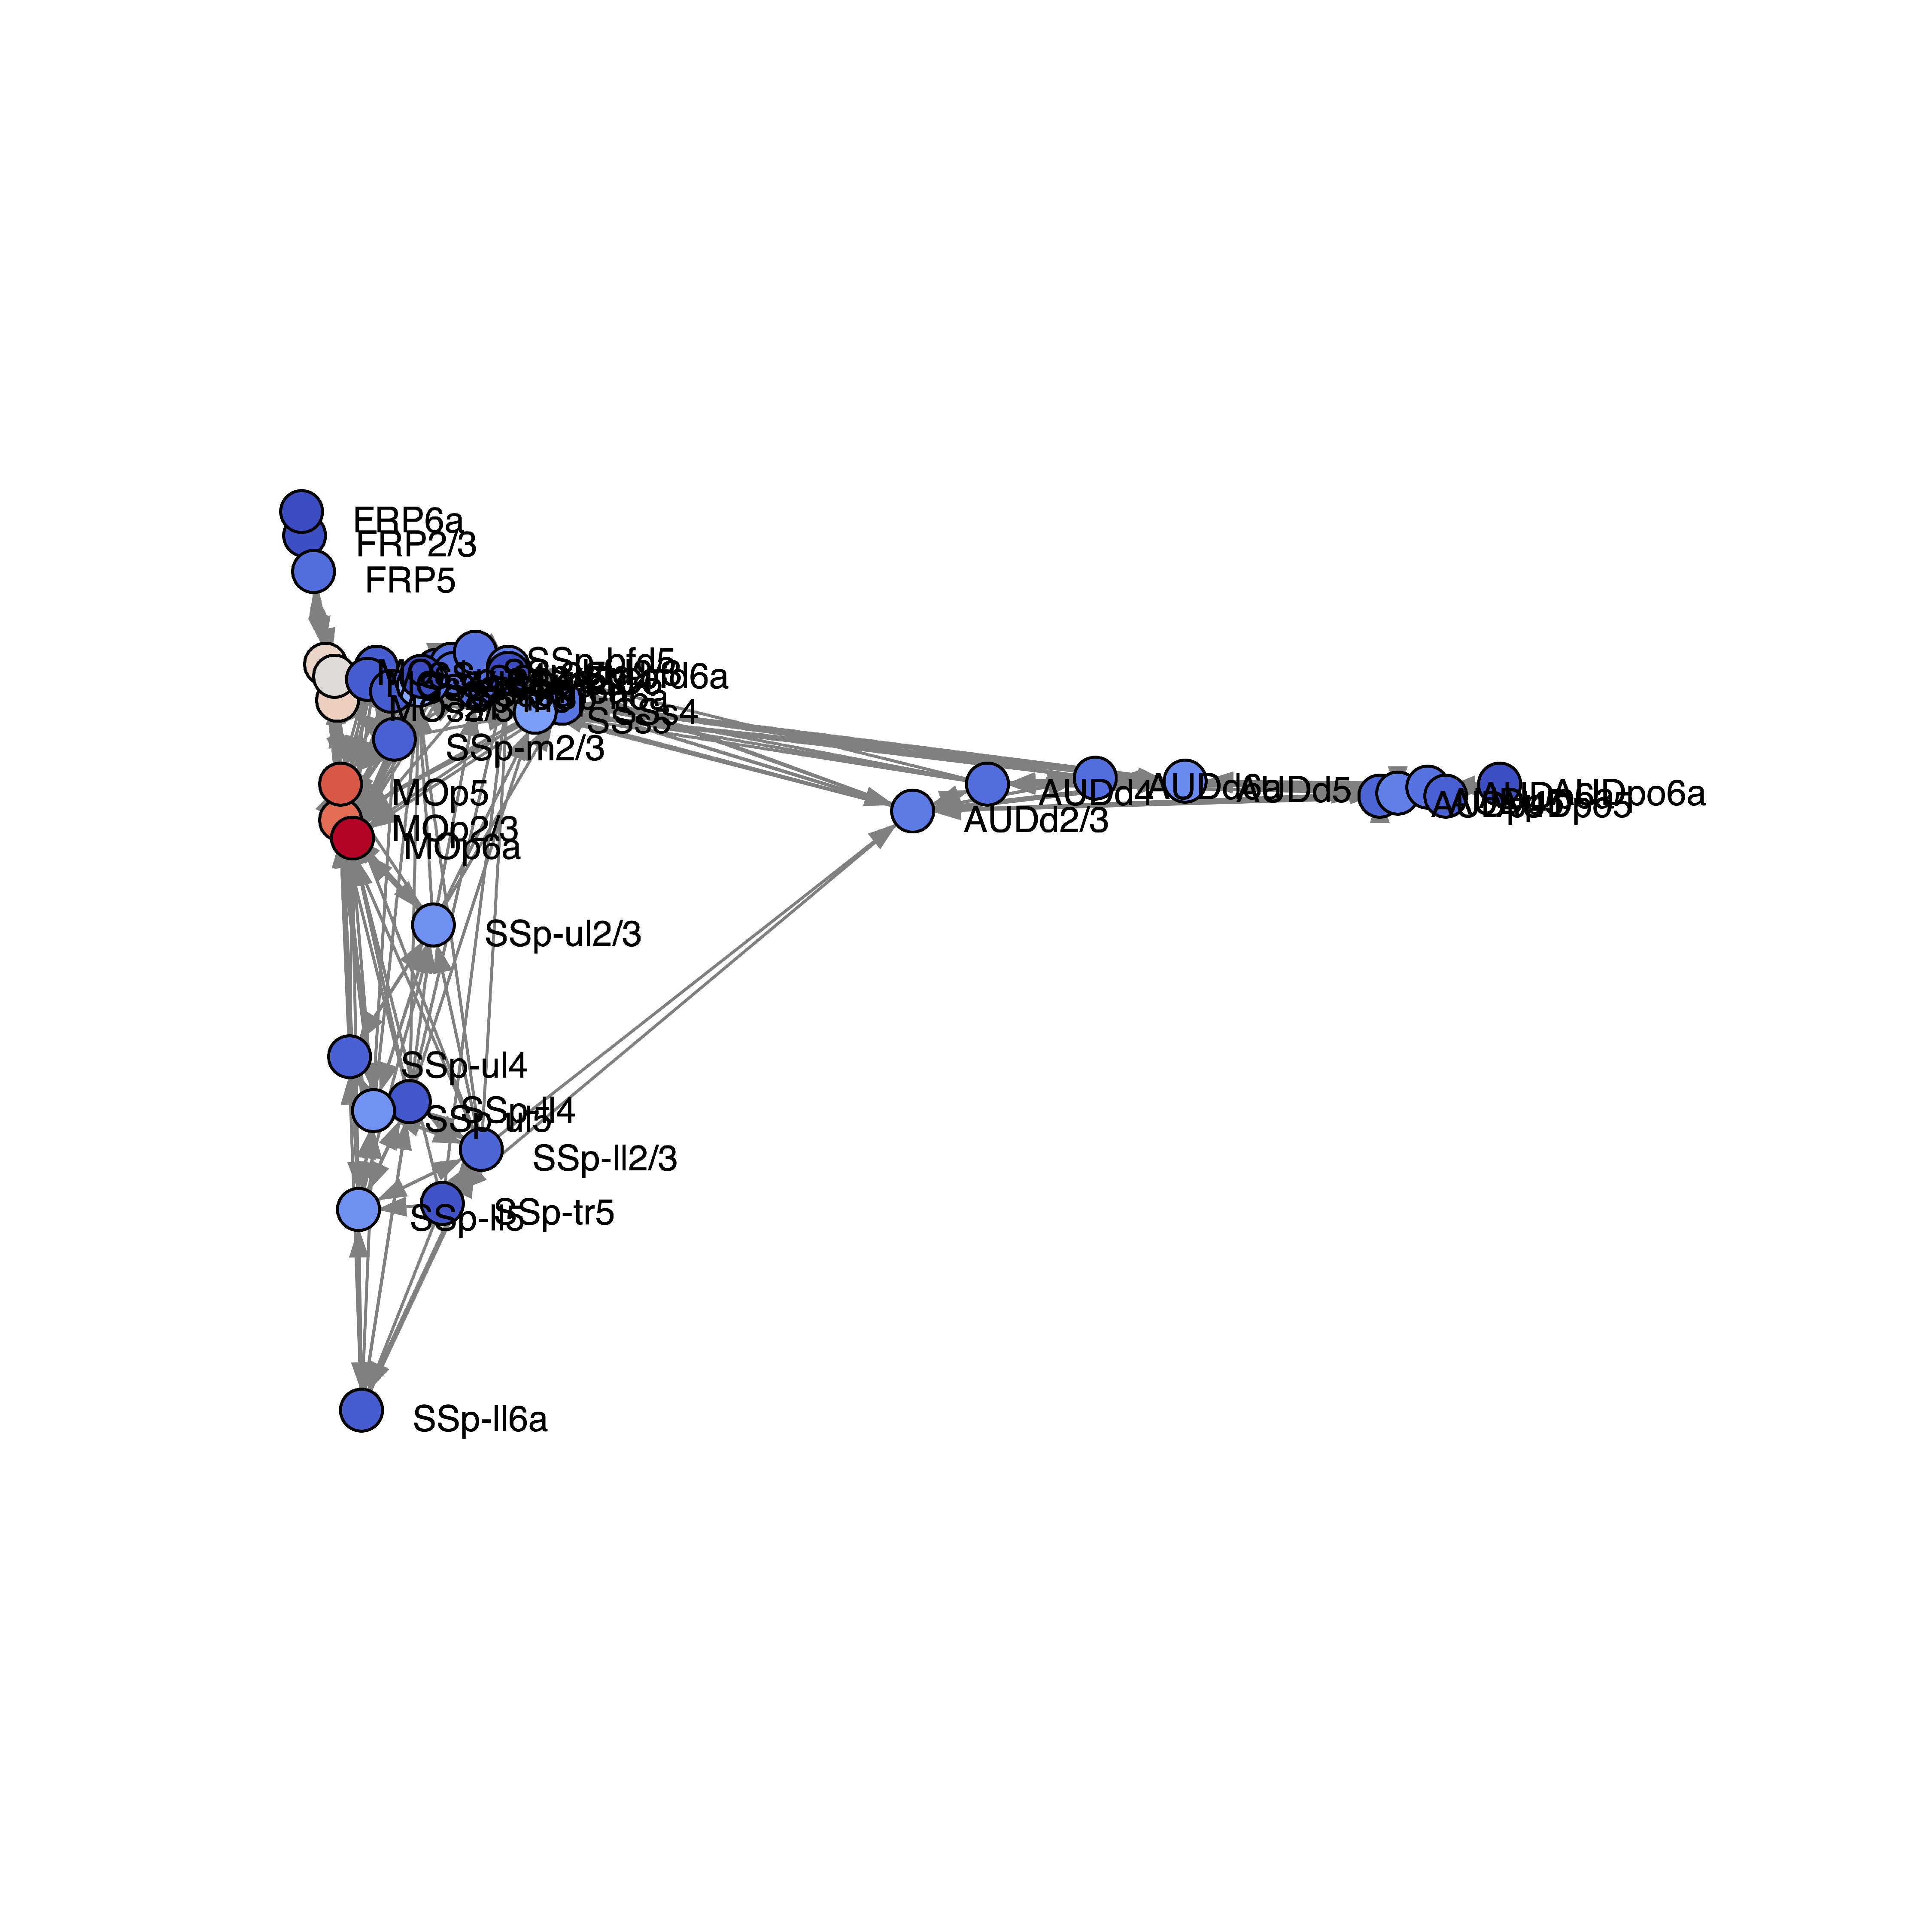
\includegraphics[width = 3in]{figs/page_graph}
    }
    }
\end{figure}

\newpage

\begin{figure}[H]
\subfloat[]{
    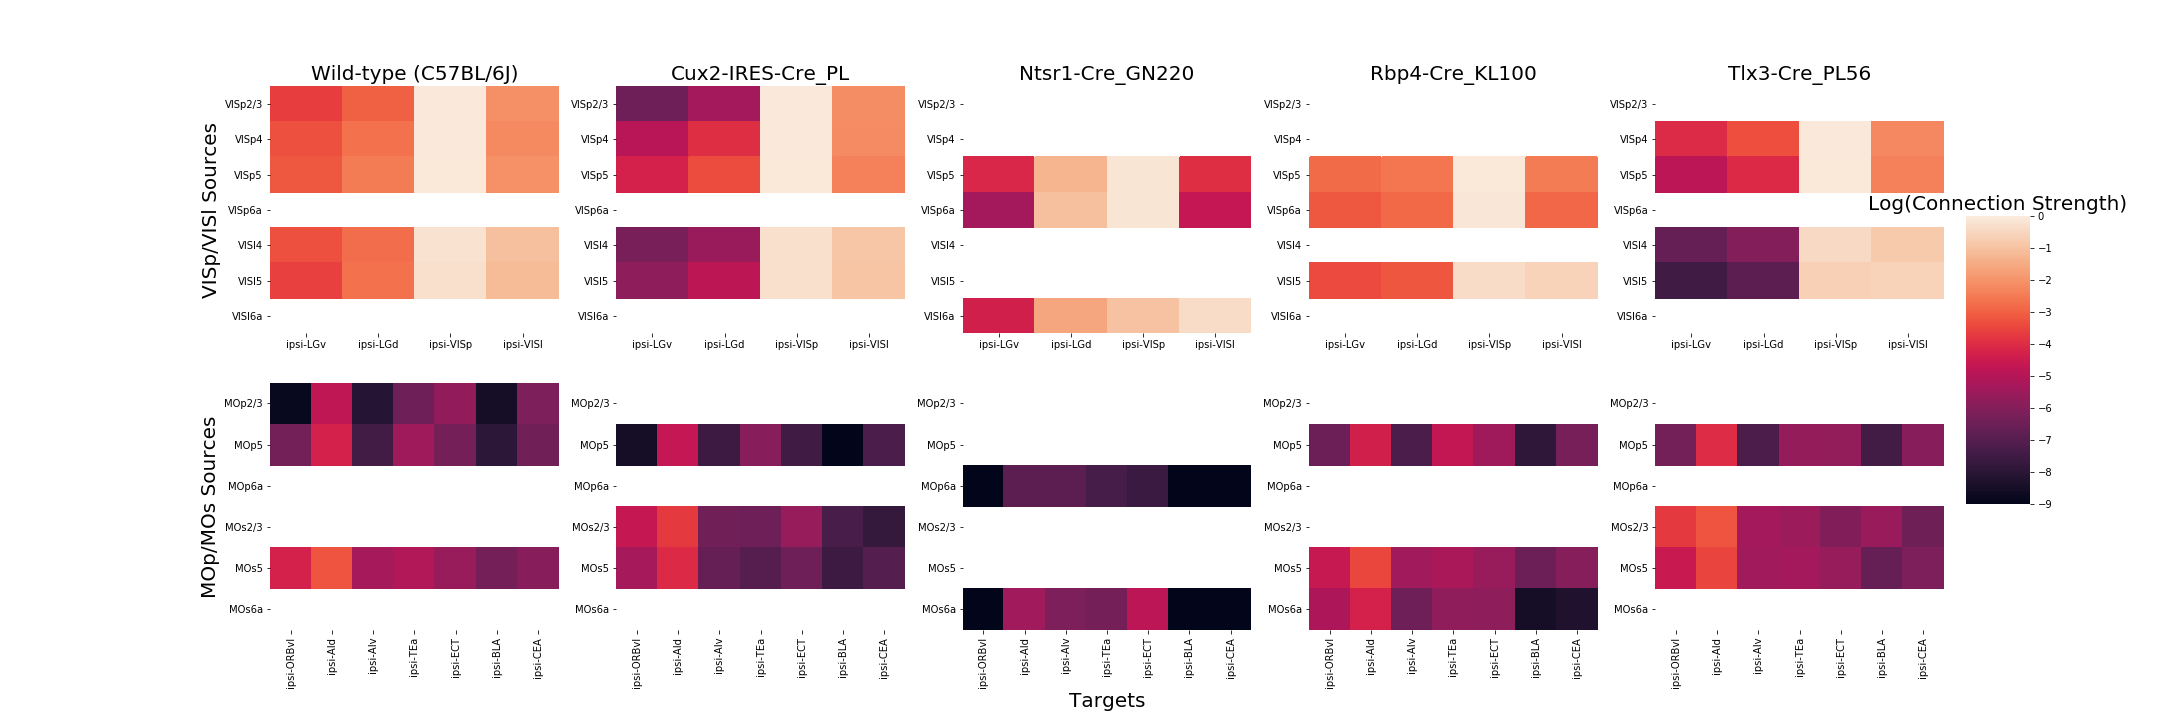
\includegraphics[width=1.\textwidth]{figs/visp_mo_1201.png}}
    \newline
 \subfloat[]{
    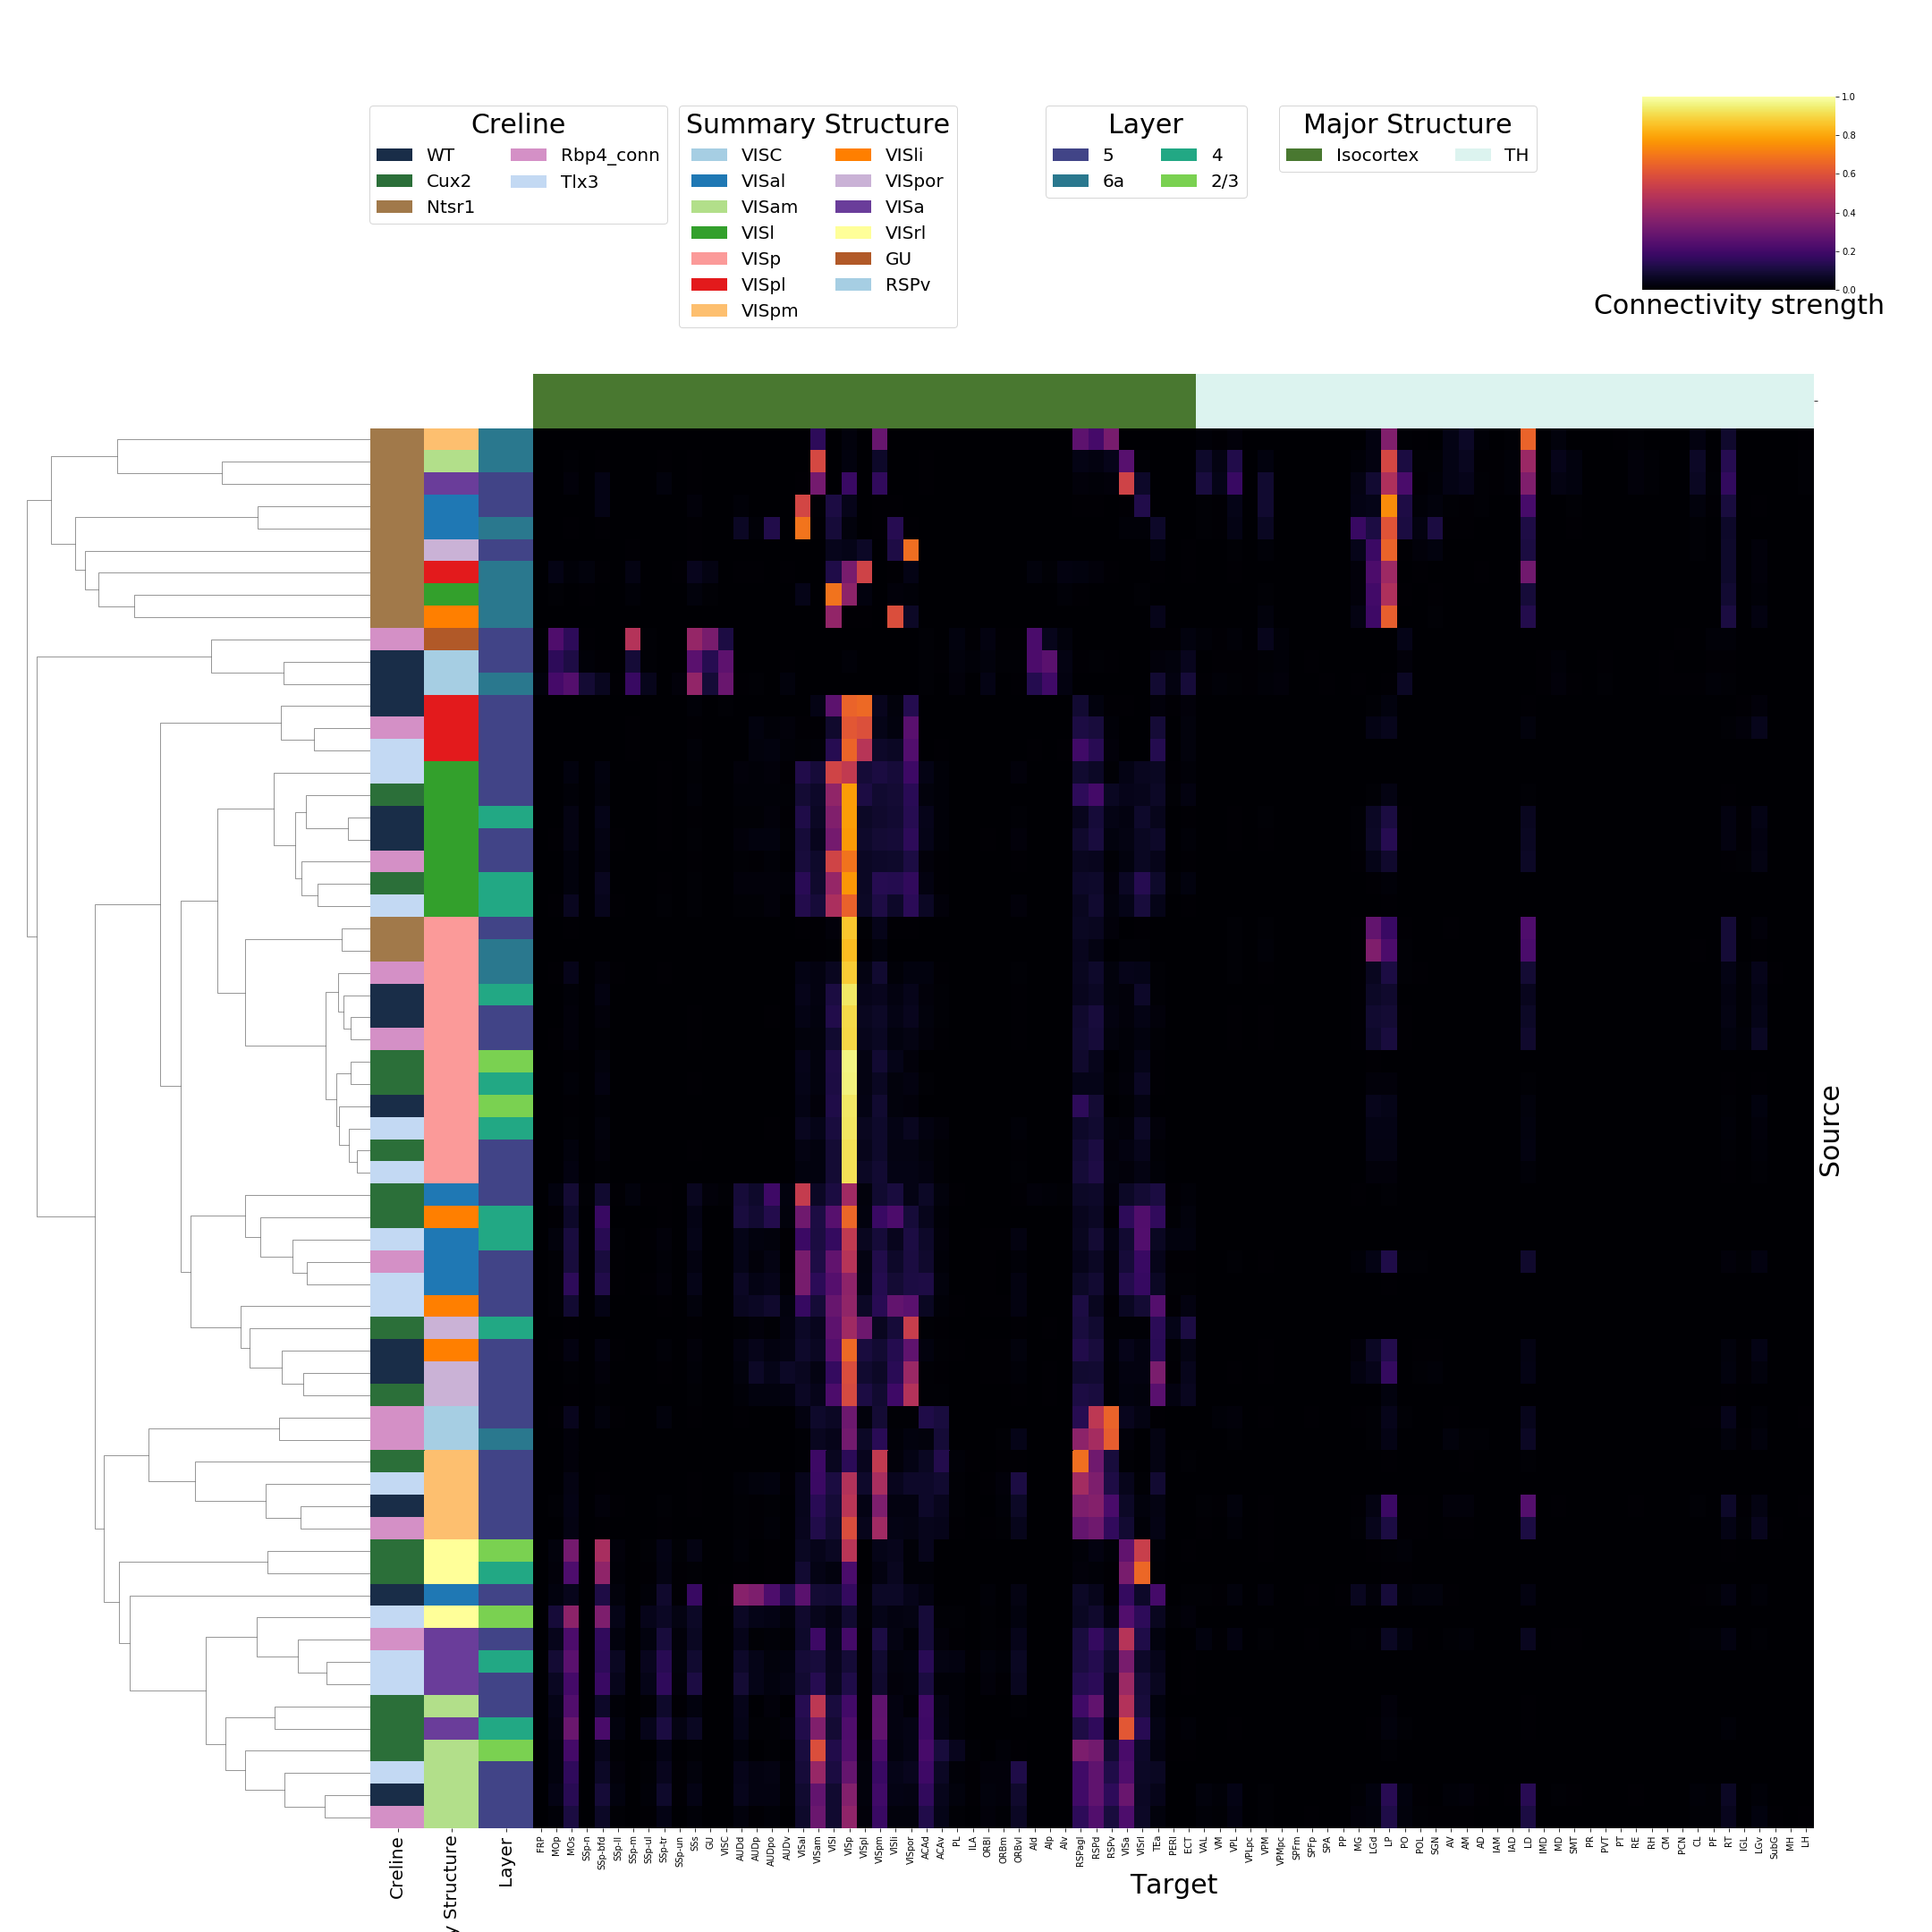
\includegraphics[width=1.\textwidth]{figs/Figure4.png}}
    \caption{   Cre-specific connection strengths from motor-cortex and visual cortex. Sources without a injection of that cre-type are blank. \skcomment{Remove 'ipsi' from columns'}}
    \label{fig:data}
\end{figure}
\newpage


\subsection{Connectivity Analyses}

%weight entropy versus accuracy

The connectivity matrix represents a collection of relatively few biological processes.
For example, certain cell-types and layers have a characteristic connectivity pattern, and structures tend to connect most strongly to the most proximal areas.
We elucidate these patterns through two types of analyses. 
First, we demonstrate cell-type specific connectivity patterns by heirarchical clustering of connectivities from multiple cre-lines, and showing that cre-line is a key factor driving the observed behavior. 
Then, we perform a different unsupervised analysis - non-negative matrix factorization - of distal wild-type connectivities, to estimate underlying overall connectivity patterns.

Figure \ref{fig:heirarchical} shows a collection of connectivity strengths generated using cre-specific models for wild-type, Cux2, Ntsr1, Rbp4, and Tlx3 cre-lines from visual signal processing leafs in the cortex to cortical and thalymic nucleii.
Heirarchical clustering is applied to sort the different source/cre combinations by the similarity of their connectivities to summary-structure targets.
This analysis shows that Ntsr1 cre-lines tend to target thalymic nucleii, in particular LP and LD \citet{Jeong2016-dc}.
However, with this exception, for the other plotted cre-lines, connectivity tends to cluster by source structure.
That the tendency for structures to connect to themselves is quite strong emphasizes the special nature of the Ntsr1-Thalymic connection in this analysis.

The overall wild-type connectivity strength matrix also displays an underlying modellable structure.
As discussed in \citet{Knox2019-ot}, one of the most basic processes underlying the observed connectivity is the tendency of each source region to predominantly project to proximal regions.
The heatmap in \ref{fig:nmf}a) shows intraregion distances clearly contains an overall pattern reminscent of the connectivity matrix in \ref{fig:connectome}.
This relationship is plotted in \ref{fig:nmf} b), showing that there exists substantial variability that would be impossible to model with low-error in a univariate model, even using the diffusion model suggested in \citet{Knox2019-ot}.
These connections are biologically meaningful, but also unsurprising, and their relative strength biases learned latent coordinate representations away from long-range structures.
For this reason, we establish a $1500 \mu m$ 'distal' threshold within which to exclude connections for our analysis.
We then apply non-negative matrix factorization (NMF) to decompose the remaining censored matrix into a relatively small number of distinct projection signals, and apply an unsupervised cross-validation method to select the optimum number of signals \skcomment{Percent error... show reconstruction? log scale?}.





%The different cre-lines display distinct connectivity patterns.


%This analysis shows that there are relatively few architypal signals underlying the overall connectome.
%Association of these patterns with the underlying biological processes is a fundamental goal in neuroscience.

%simply exhibit a collection of these patterns using several factorization methods applied to the connectivity matrix $\mathcal C$.

%Since much of the connectivity matrix can be predicted solely based off of location information.  For this reason, we subtract our the simple $\hat f_{d} c(p_1), c(p_2)$ where $\hat f$ is the estimated relation of distance between regional centroids and connectivity strength.

%, which we elucidate through n. First, projection signals cluster by target and by source; we can identify similarly behaving structures and neural targets that tend to co-occur.  Second, the specific cell-types targeted by the various cre-lines themselves generate a reduced-dimension space. Under the assumption that cell-type determines projection pattern, we can investigate which cell-types are present in which of the projecting structures.

%The choice of matrix factorization method reflects particular scientific subquestions and probabilistic interpretations. 

\newpage

\begin{figure}[h]
    \centering
    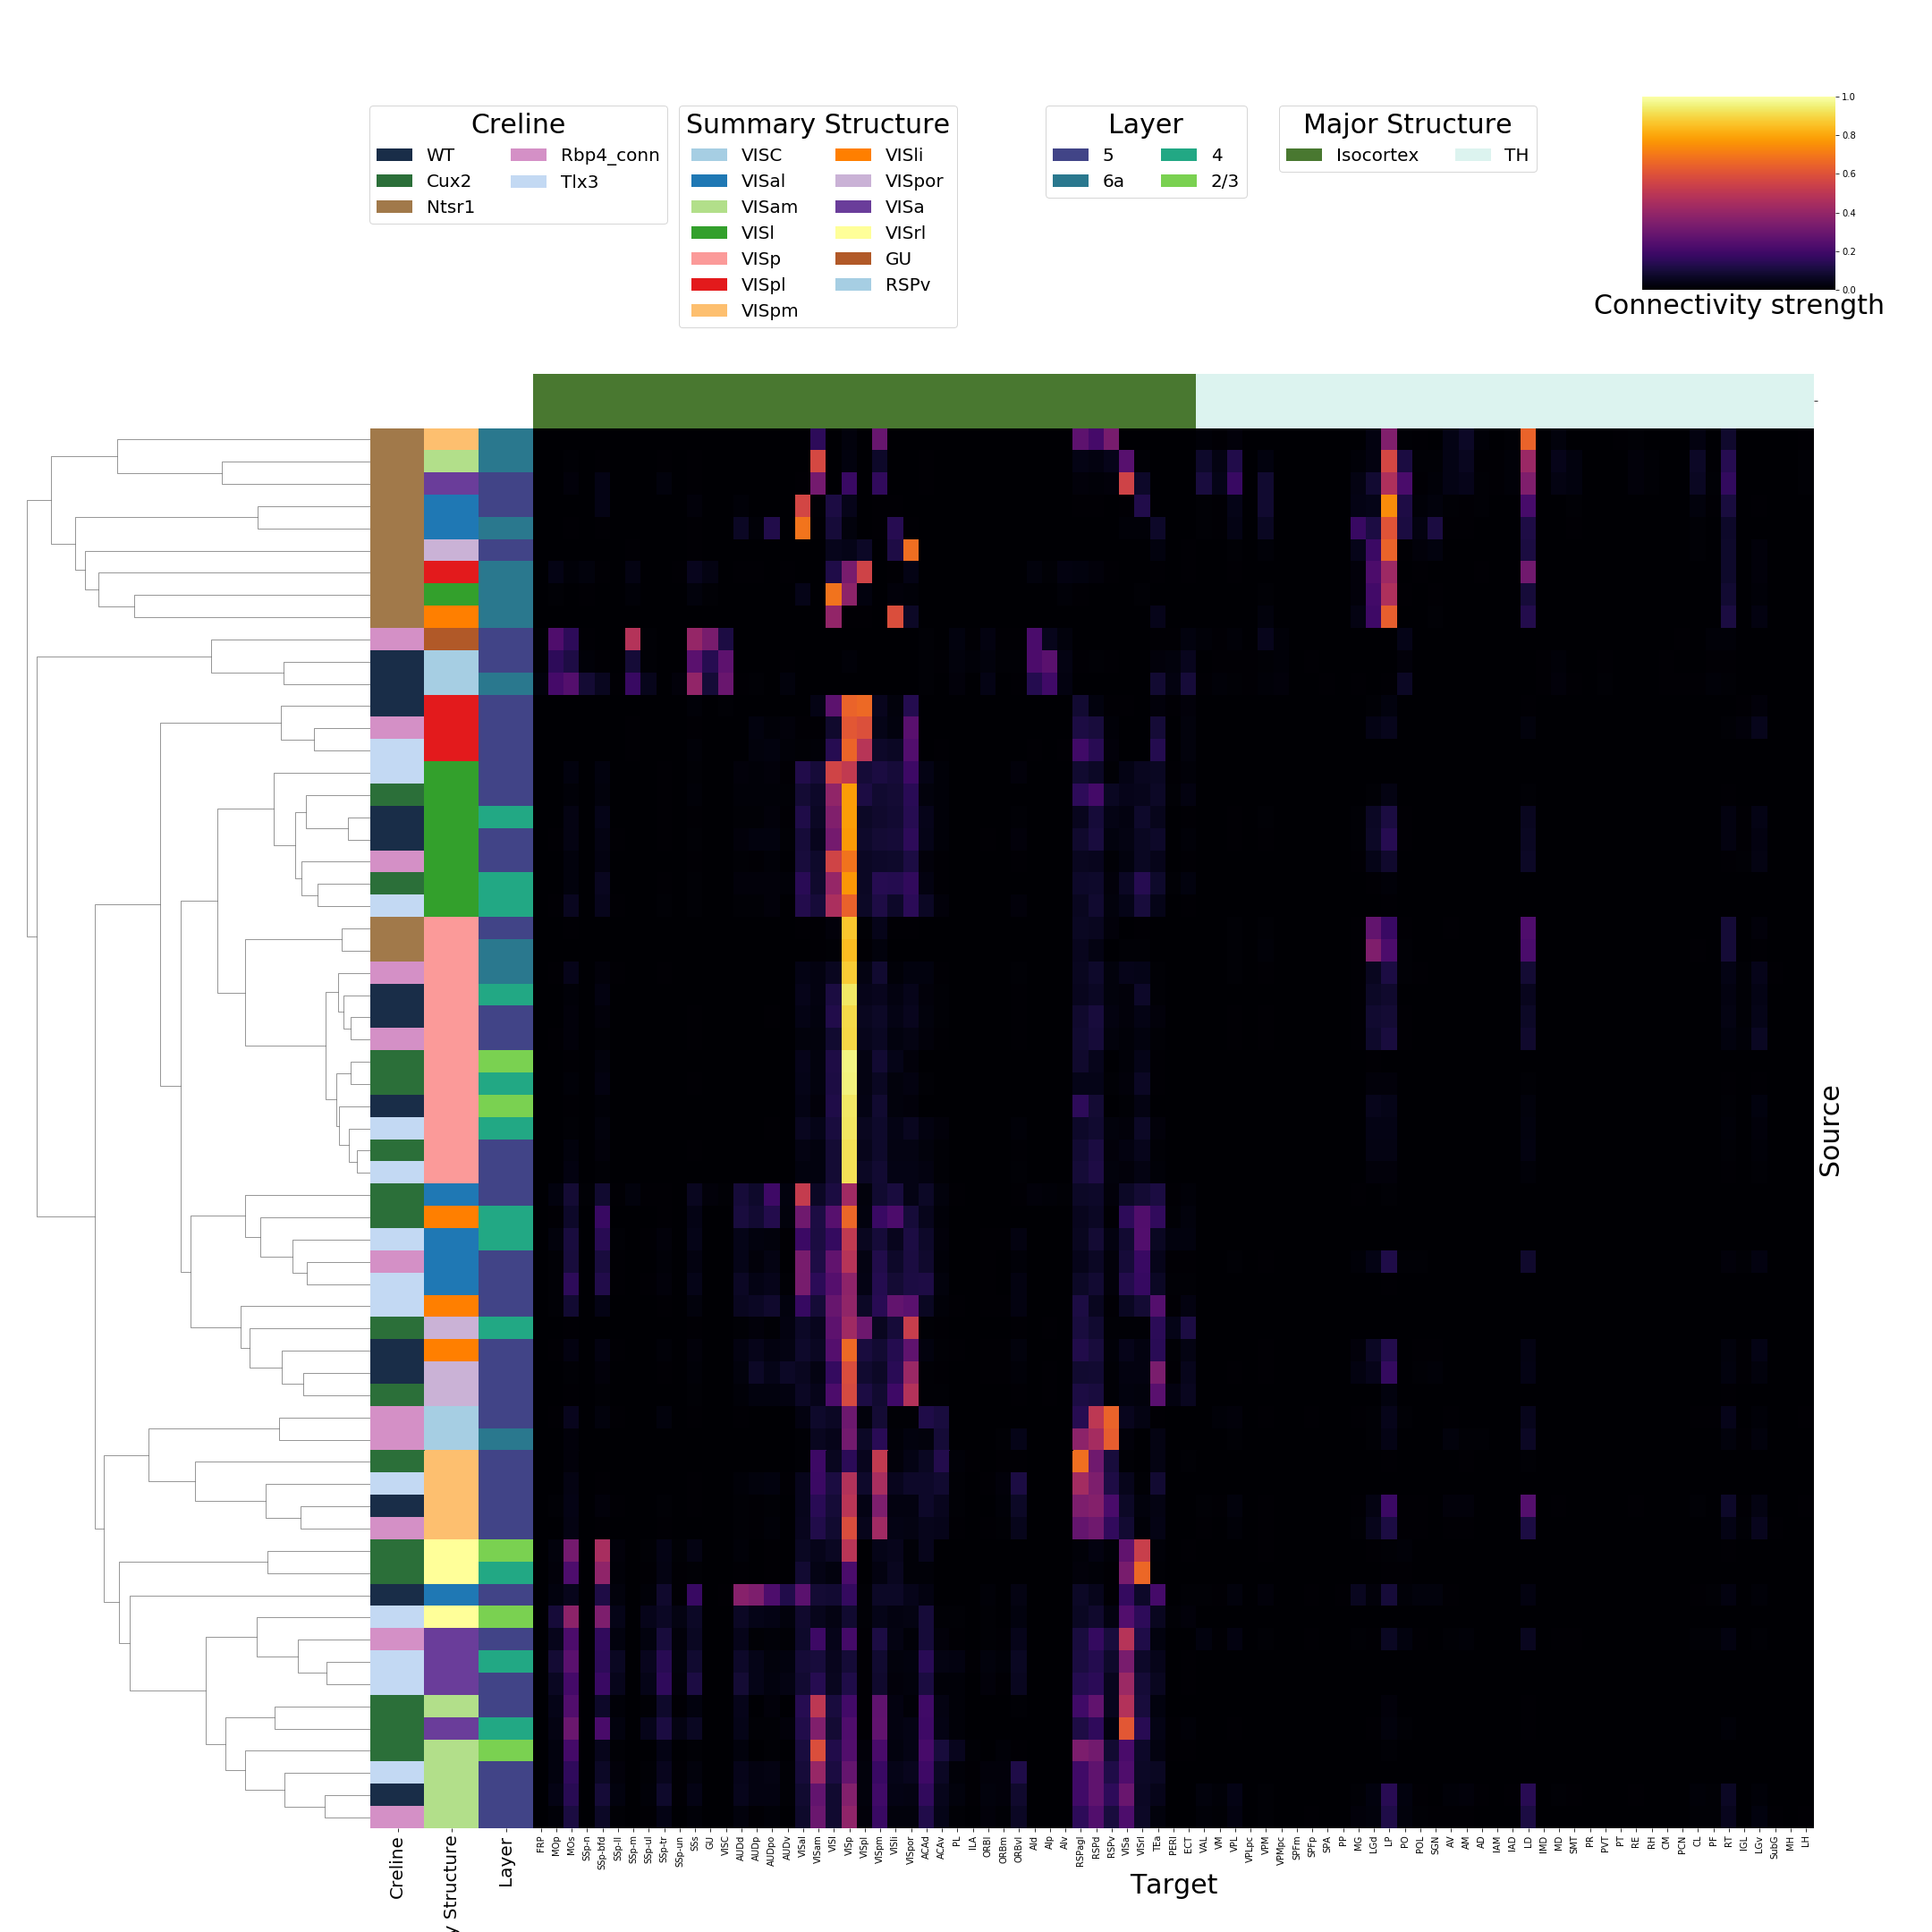
\includegraphics[width = 6in]{figs/Figure4.png}
    \caption{Heirarchical clustering of connectivity strengths from visual signal processing cell-types to cortical and thalymic targets. Cre-line, summary structure, and layer are labelled on the sources. Note that sources/cre combinations are only included if there is at least one experiment of that cre-line in that particular leaf.}
    \label{fig:heirarchical}
\end{figure}
\newpage

\begin{figure}[h]
\begin{tabular}[t]{ccc}
\subfloat[]{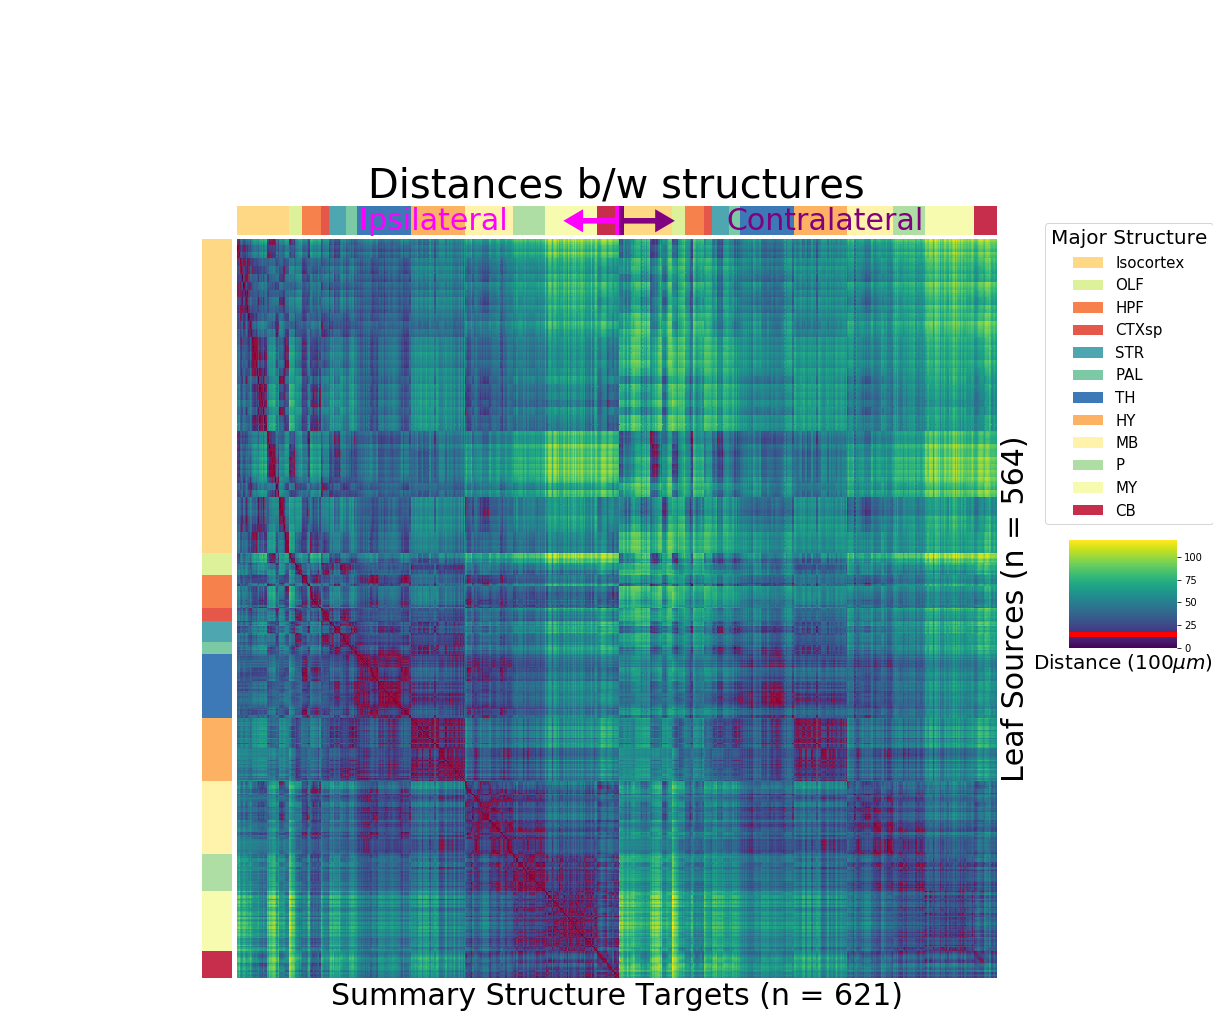
\includegraphics[width = 2in]{figs/distances_nice.png}}
& 
\vspace{1cm}
\subfloat[]{\includegraphics[width = 1.5in]{figs/figsforpres/test_train.png}} &
\subfloat[]{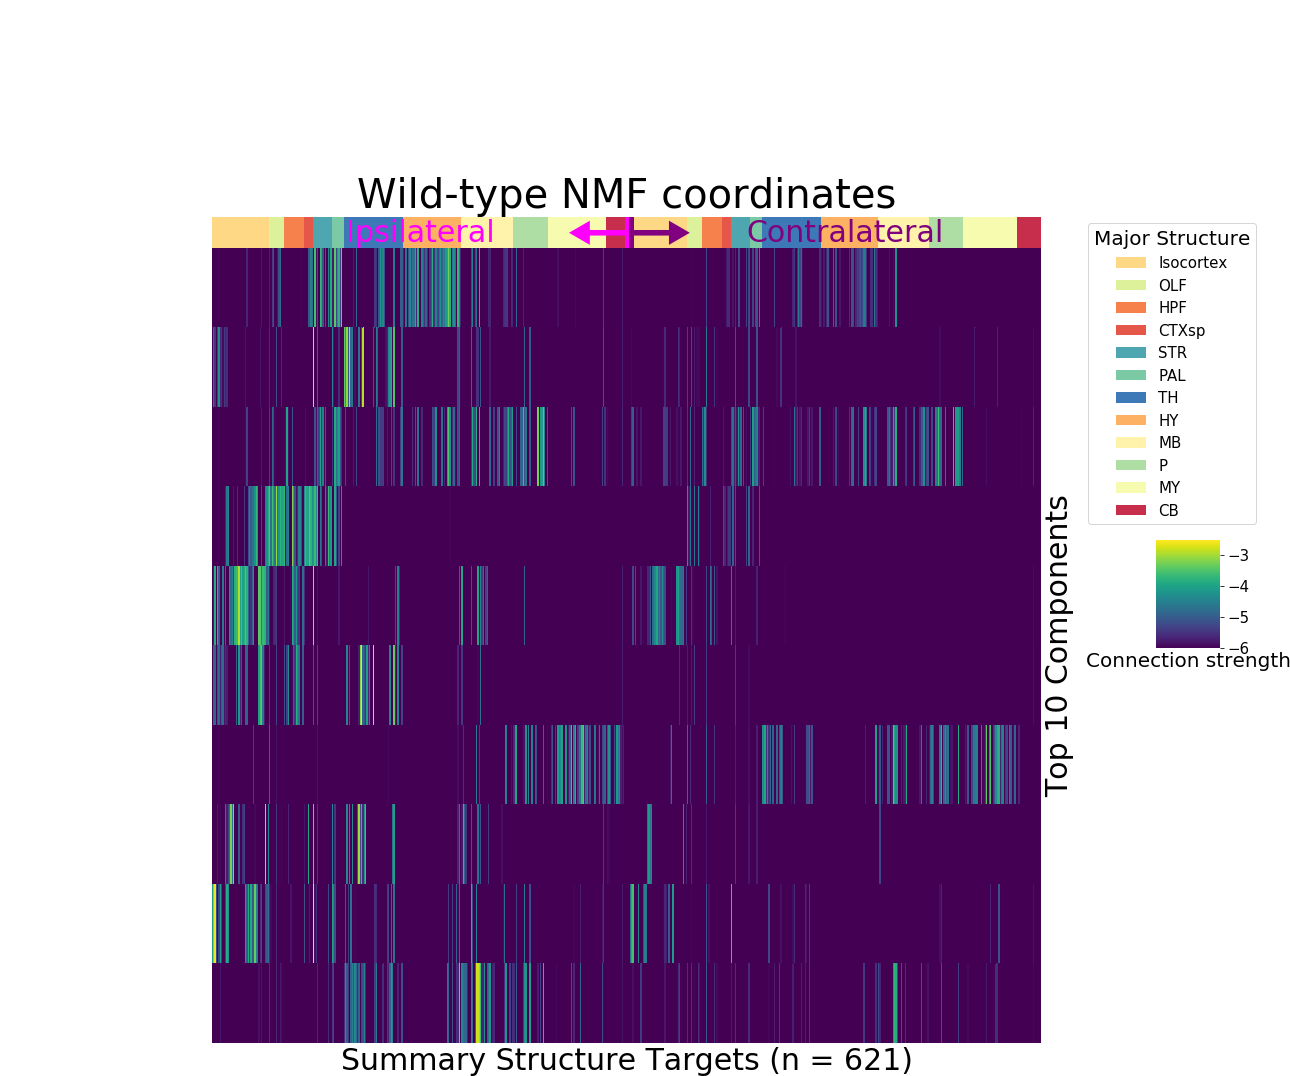
\includegraphics[width = 2in]{figs/wt_nmf_alpha0.png}}
\end{tabular}
\end{figure}

\begin{figure}[h]
    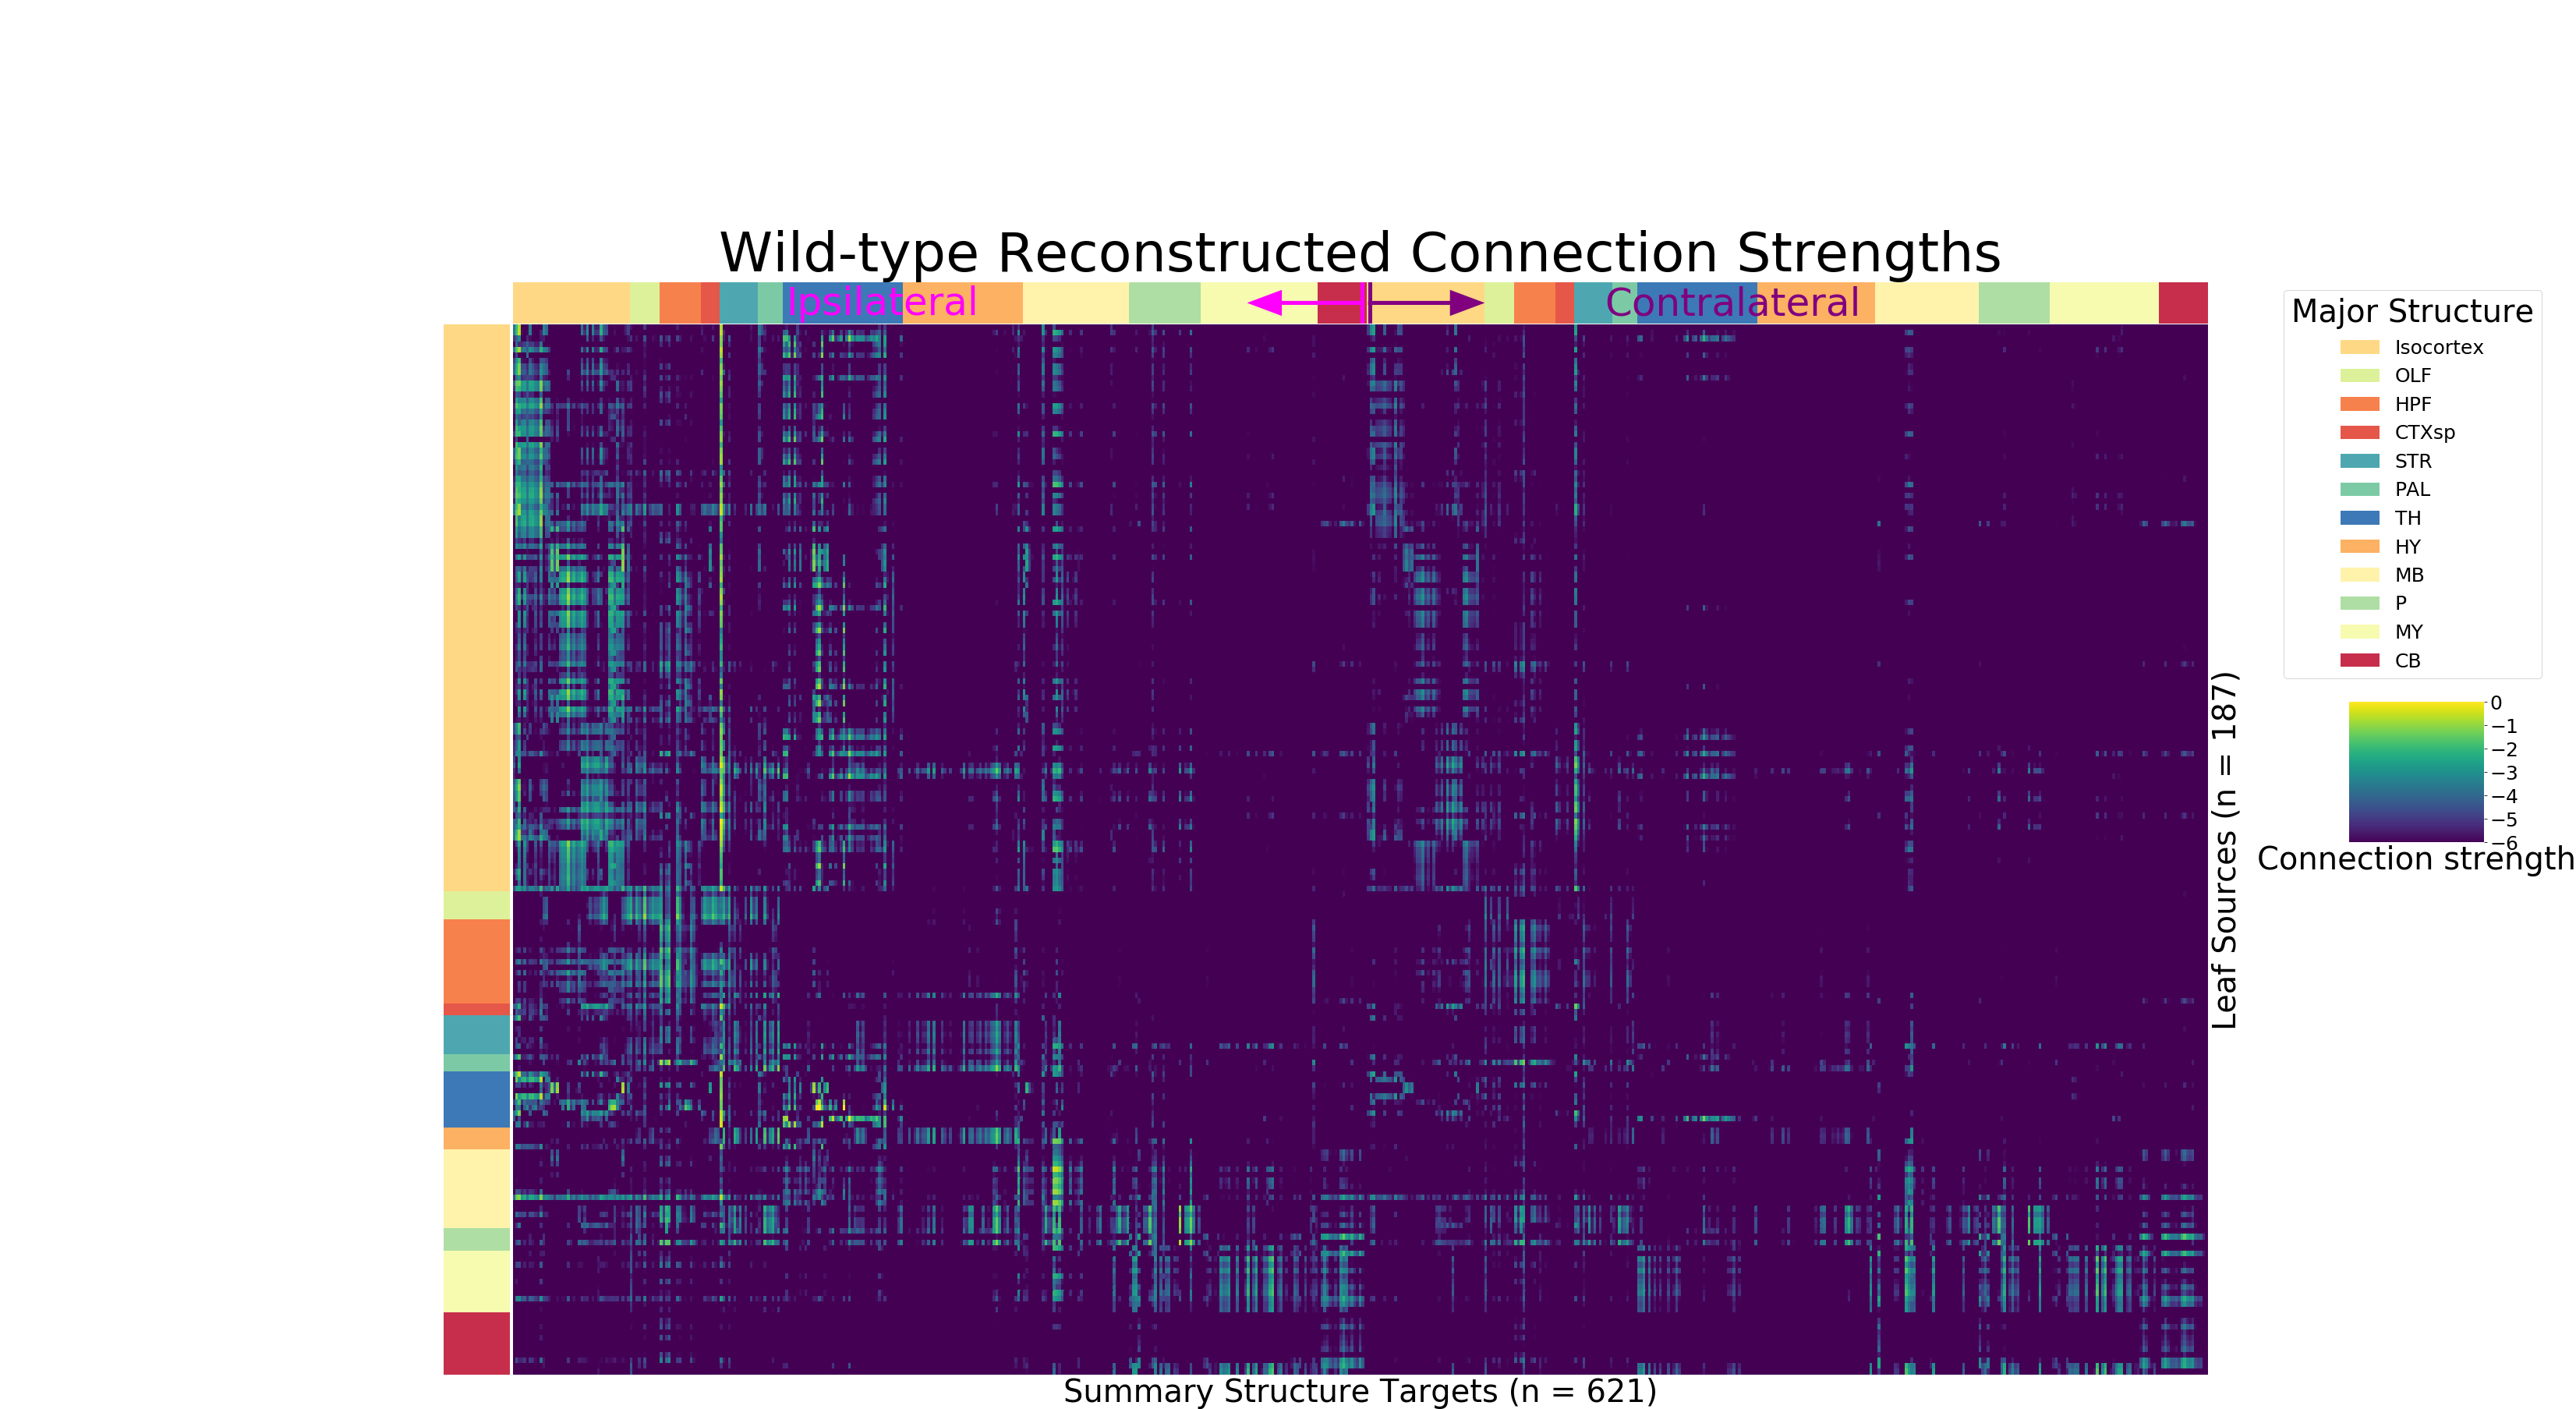
\includegraphics[width = 5in]{figs/wt_recon.png}
    %\caption{Caption}
    \label{fig:my_label}
\end{figure}
% \begin{figure}[h]
%     \centering
%     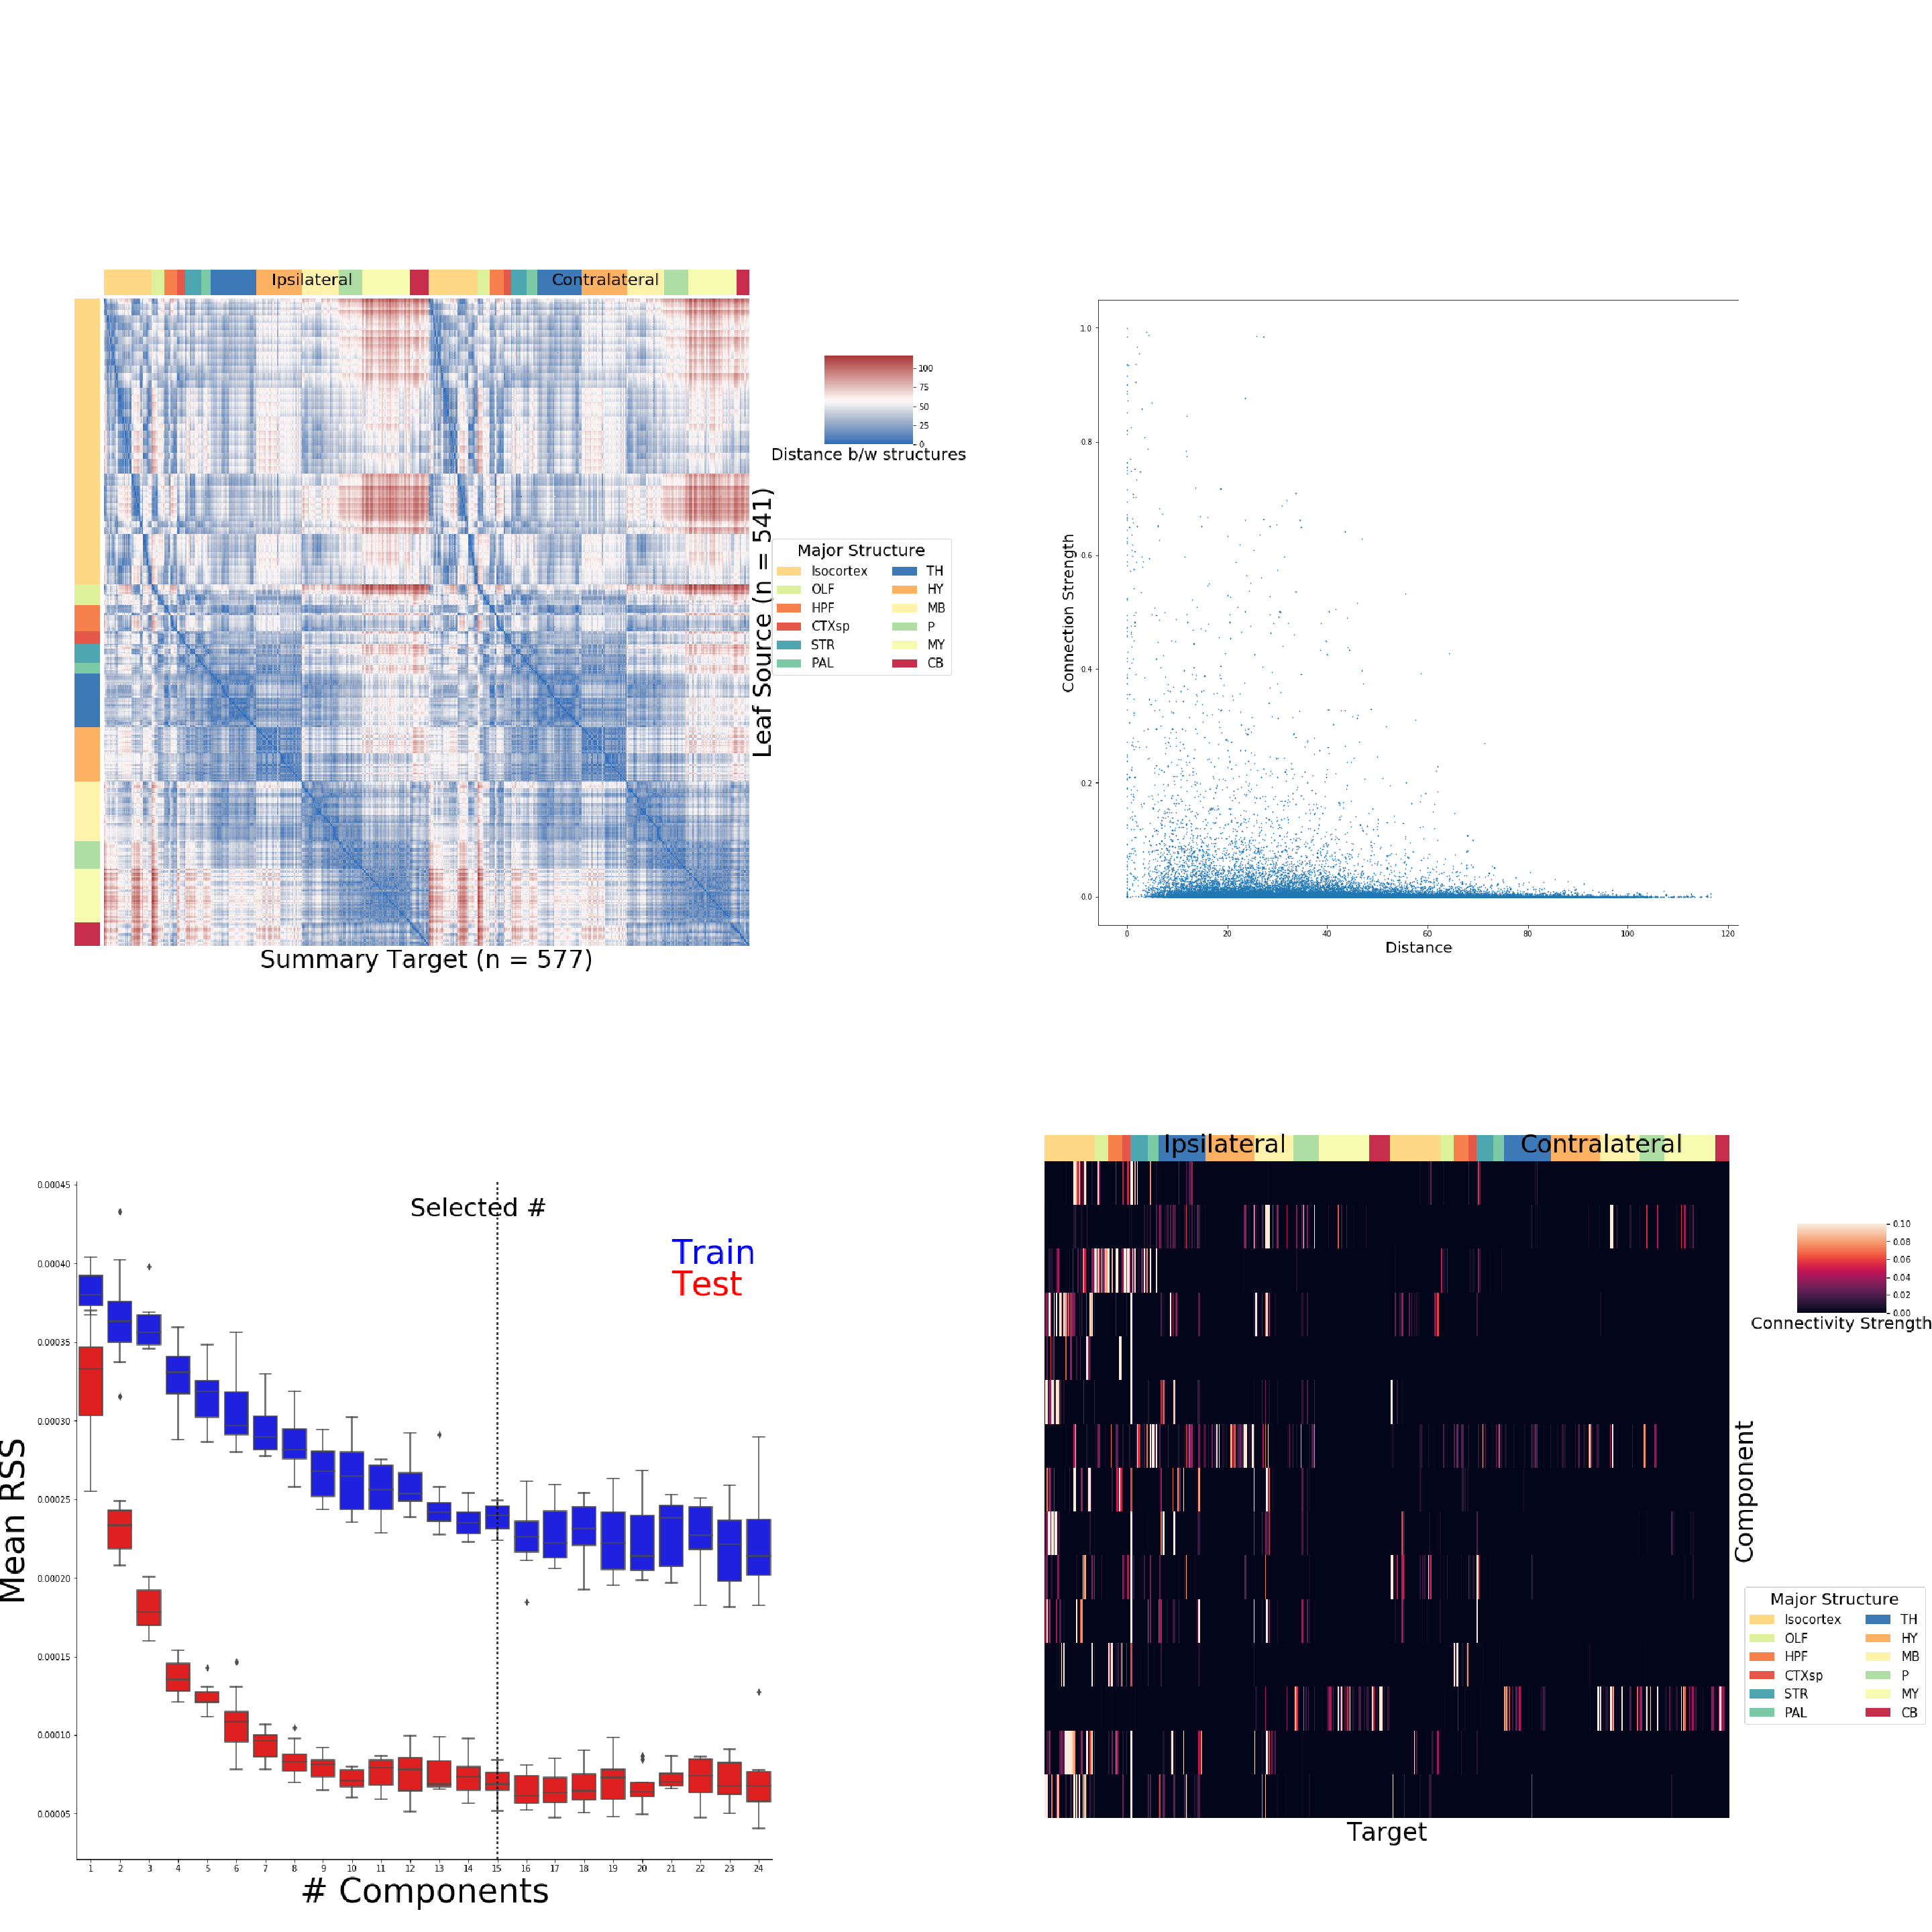
\includegraphics[width = 6in]{figs/Figure5.png}
%     \caption{a) Distances between structures \skcomment{Add units to distance legend}. b) Relation between connectivity strength and distance. c) Train error and test error of non-negative matrix factorization of non-local ($> 1500 \mu m$) connectivities. d) The top $15$ factorization components. \skcomment{Why is compressability so high}}
%     \label{fig:nmf}
% \end{figure}
% \newpage





%Our core model evaluation method is leave-one-out cross validation. This method is robust to the trivial overfitting in Nadaraya-Watson bandwidth selection. We show that incorporation of cre lines improves model performance in the following experimental set-ups. This requires at least two experiments in every experimental division, even in the 2-stage model, since leave-one-out means of each cre line may only be computed for cre-lines which are present at least twice in the leaf. This is the set up for a model trained on all data. However, for alternate models, such as the major-structure divided model from \citet{Knox2019-ot}, the potential evaluation set is larger. In order to compare between methods, we therefore restrict to the smallest set of evaluation indices, which is to say, virus-leaf combinations that are present at least twice.  This means that in some cases, our training set exceeds our evaluation set in size. 


%\begin{tabular}{lrrrr}
%{} &  Jackknife 2-stage &  Leaf average &  Creleaf average &  Creleaf NW \\
%Isocortex &           0.247344 &      0.495706 &         0.336688 &    0.300725 \\
%OLF       &           0.355304 &      0.415619 &         0.511035 &    0.550080 \\
%HPF       &           0.175599 &      0.288700 &         0.244325 &    0.252792 \\
%CTXsp     &           0.444341 &      0.444341 &         0.444341 &    0.444341 \\
%STR       &           0.339494 &      0.876627 &         0.386912 &    0.407204 \\
%PAL       &           0.221939 &      0.414942 &         0.299539 &    0.301274 \\
%TH        &           0.333870 &      0.403145 &         0.644163 &    0.644865 \\
%HY        &           0.219867 &      0.260841 &         0.303319 &    0.294789 \\
%MB        &           0.254503 &      0.431675 &         0.310175 &    0.264034 \\
%P         &           0.183399 &      0.296101 &         0.240284 &    0.240284 \\
%MY        &           0.133392 &      0.260755 &         0.316030 &    0.291915 \\
%CB        &           0.113383 &      0.565529 &         0.148914 &    0.148914 \\
%\end{tabular}


%\begin{table}[]
%    \centering
%\begin{tabular}{l|r|r|r}
%{} &         New model & Cre-specific old model & Old model\\
%Isocortex  &  0.127336 &  0.150736 &    0.184242  \\
%OLF  &  0.058567 &  0.079846 & 0.077752 \\
%HPF  &  0.079664 &  0.108270 & 0.128780\\
%CTXsp  &  0.496673 &  0.496673 & 0.496673 \\
%STR  &  0.051538 &  0.067820 & 0.081748\\
%PAL  &  0.135417 &  0.195684 & 0.256060 \\
%TH  &  0.319509 &  0.573850 &  0.314612\\
%HY  &  0.209917 &  0.259324 &  0.233678\\
%MB  &  0.112262 &  0.119420 &  0.121561 \\
%P  &  0.226793 &  0.238584 &  0.257031\\
%%MY &  0.158823 &  0.238236  &  0.193499 \\
%CB &  0.040000 &  0.049516 & 0.064922 \\
%\end{tabular} 
%\caption{Caption}
%    \label{tab:my_label}
%\end{table}


%\begin{tabular}{lr}
%{} &    Old model  \\
%0  &  0.184242 \\
%1  &  0.077752 \\
%2  &  0.128780 \\
%3  &  0.496673 \\
%4  &  0.081748 \\
%5  &  0.256060 \\
%6  &  0.314612 \\
%7  &  0.233678 \\
%8  &  0.121561 \\
%9  &  0.257031 \\
%10 &  0.193499 \\
%11 &  0.064922 \\
%\end{tabular}



% \begin{figure}[H]
%     \centering
%     \includegraphics[width = 10cm]{Figures/Connectivities/wildtype.png}
%     \caption{Caption}
%     \label{fig:wt_visp_conn}
%     %this is the old figure... update
% \end{figure}

%\begin{figure}[p]
%    \centering
%    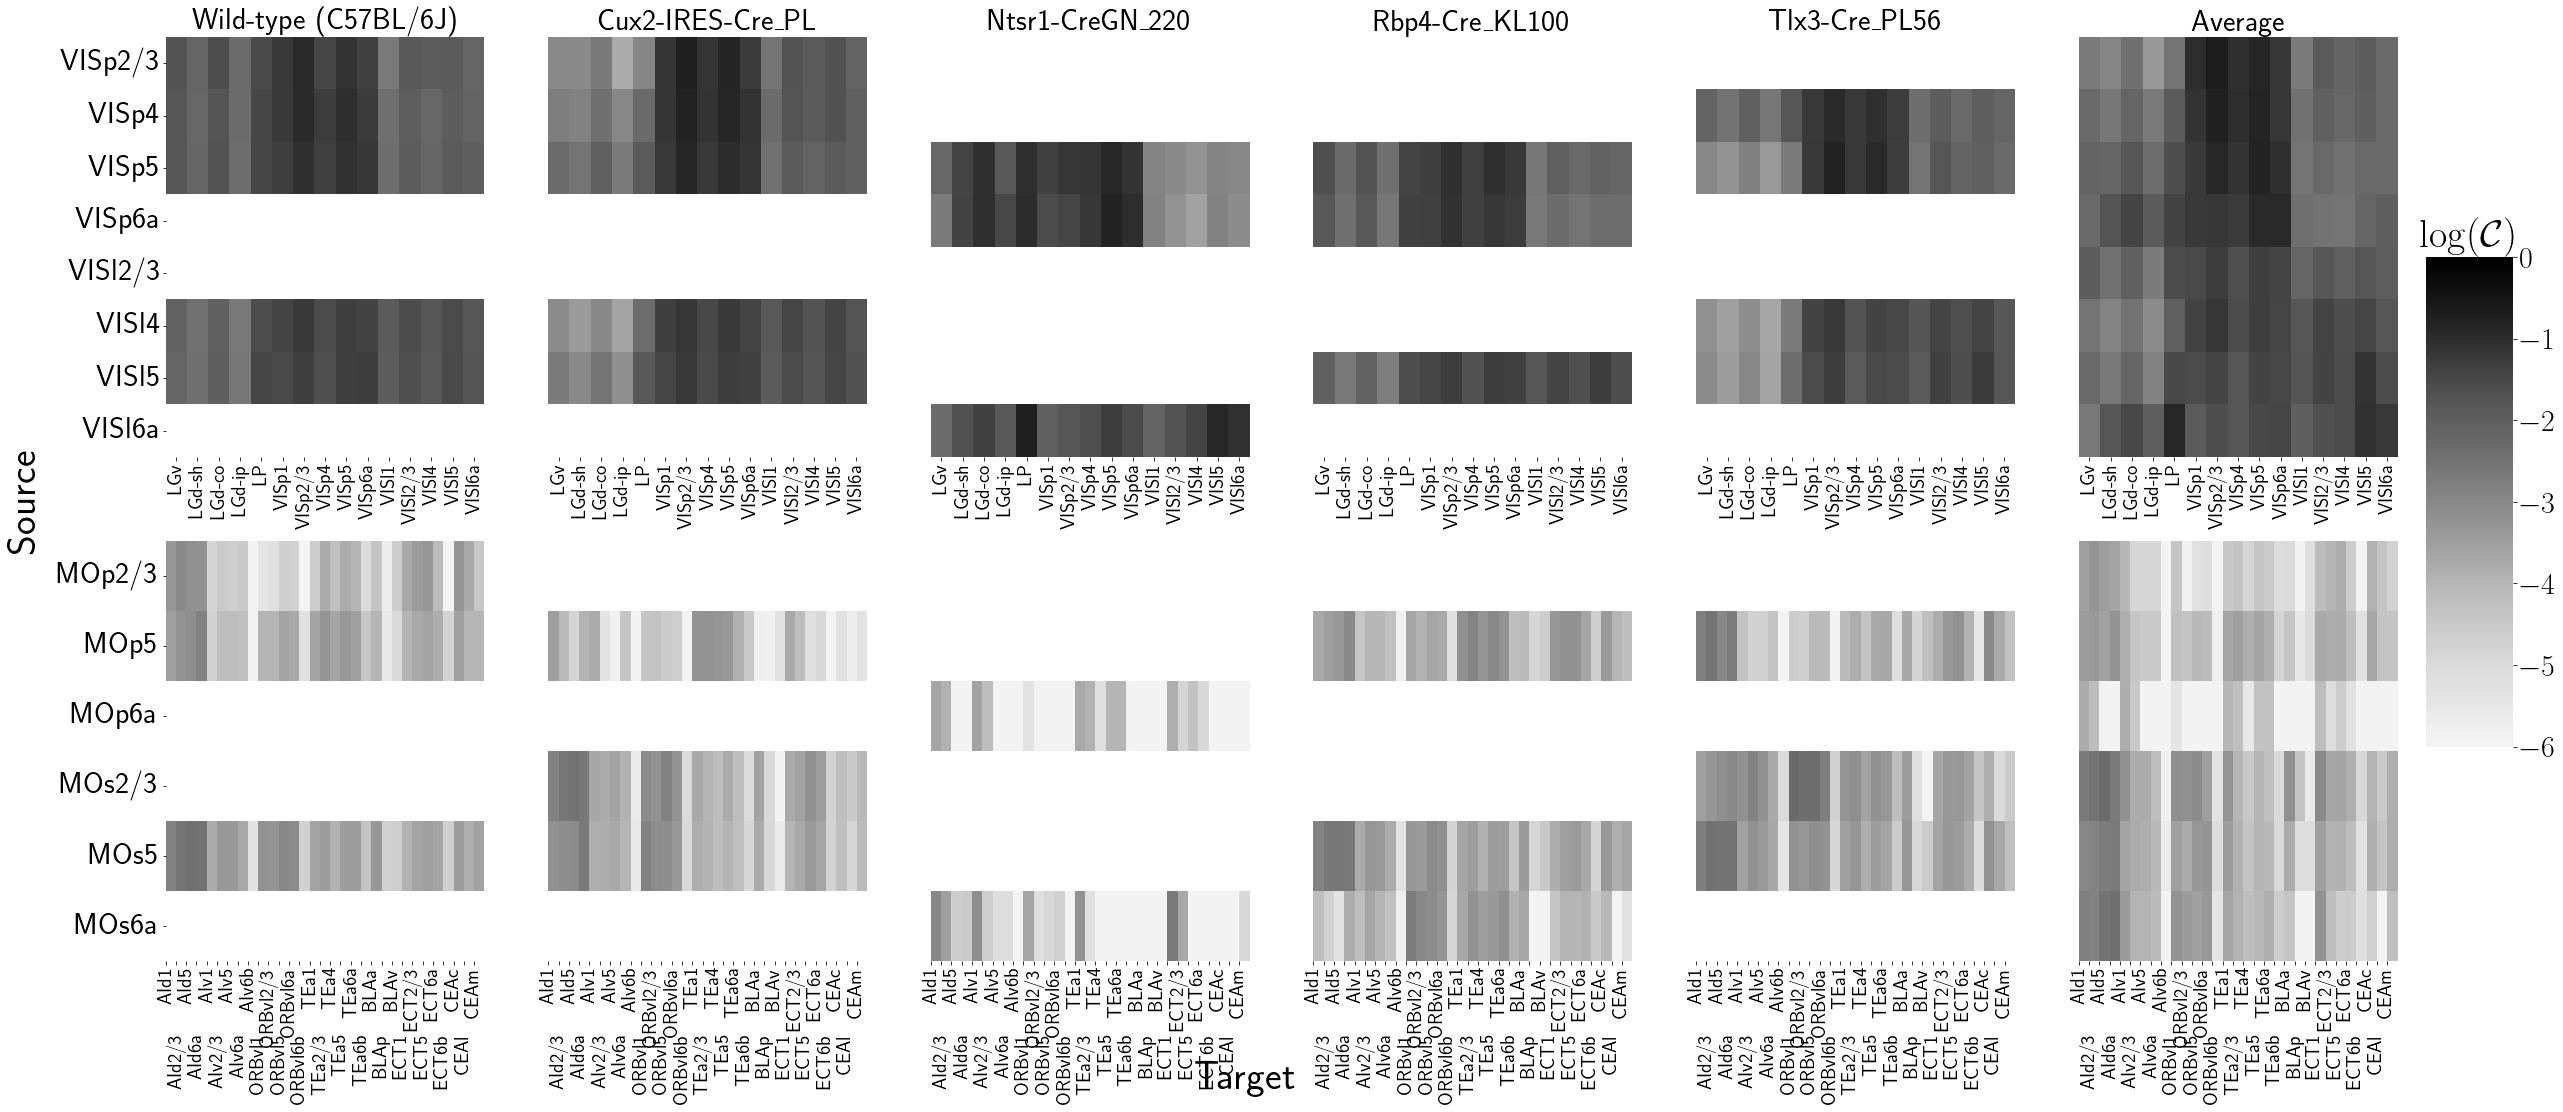
\includegraphics[width = 18cm]{figs/visp_mo.png}
%    \caption{Cre-line specific connectivity matrices for a selection of sources and targets are displayed as heatmaps. Sources without a injection of that cre-type are blank.}
%    \label{fig:my_label}
%\end{figure}


\section{Discussion}

Flattening $\mathcal C$ prior to unsupervised analysis is not necessarily recommended, but provides an easy solution for this problem.

With respect to the model, a Wasserstein-based measure of injection similarity per structure would combine both the physical simplicity of the centroid model while also incorpating structural knowledge.

The Nadaraya-Watson weighting procedure introduced here is, to our knowledge, novel.  In particular, our method of utilizing the expected loss to weight points differs from the minimization task of fitting data to weighted sums of neighbors \citep{Saul2003-th}.  We make a key assumption: that the additional statistical accuracy of including more samples makes up for the fact that their expected accuracy is lower. Note that this assumption can be easily violated, if, for example, the data is distributed on a circle without error, and only nearest neighbors are most predictive.

Model averaging based off of cross-validation has been implemented in \citet{Gao2016-qe}, but we note that our approach makes use of a non-parametric estimator, rather than an optimization method for selecting the weights.  \skcomment{CITE METHOD THAT SELECTS WEIGHTS IN KERNEL (has catchy name)}

%and is related to the theoretical research problem of interpreting learned dynamical systems. 



%We synthesize the two equivalently in a product space as
%\begin{eqnarray*}
%d(i,i')^2 = \|\mu (v(i)) - \mu (v(i')\|_2^2 + \|c(i) - c(i')\|_2^2.
%\end{eqnarray*}

%However, the weighting of the two feature types is unclear. In lieu of an optimization-based approach for learning the weights of each distance coordinate, we utilize the following approach.

%(indeed, only wild-type tracing experiments were 


%where
%\begin{equation}
%f: \mathbb R^3 \times \mathcal V \to \mathbb R^{S_{IMC}}
%\end{equation}
%is the projection of a particular voxel.


%We therefore write the generic model with errors-in-variables as
%The general model is thus

%\begin{eqnarray*}
%y = f(x + \epsilon_x, v) + \epsilon_y.
%\end{eqnarray*}

%We assume $\epsilon_x = 0$, and $x$ and $y$ have been regionalized as $r_y(y(i)) \in \mathbb R^{S_{IMC}}, r_x(x(i) \in \mathbb R^S$. \citet{Knox2019-ot} utilizes the model $r(y(i)) = f_{NW} (c(x(i)))$, where $f_{NW}$ is the Nadaraya-Watson estimator.  In contrast, \citet{Oh2014-kh} uses the model $r(y(i)) = f_{NNLS} (r(x(i)))$ where $f_{NNLS}$ is fitted non-negative least squares.  In both cases, data consisted of only the wild type cre line.
%Although the Knox model is conceptually simpler, it generated improved predictive performance. This improvement is due to the fact that the regionalization map $r$ is a relatively coarse description of the injection $x(i)$, compared with the centroid function $c(x(i))$.  Furthermore, the slow convergence of the Nadaraya-Watson estimator is mediated by the lower dimensionality of $c(x(i))$ compared with $r_x x((i))$, and generalization issues caused by poor-conditioning of the somewhat sparse design matrix $r(x(1:n))$ are avoided.

%The major-structure specific Nadaraya-Watson estimator from $\citet{Knox2019-ot}$ nevertheless appears poorly adapted for our circumstances since it does not take into account the virus $v$. It is not straightforward to include the viral strain in either $f_{NW}$ or $f_{NNLS}$. For $f_{NW}$, it is not clear how a one-hot encoded class-membership feature should be weighted. For $f_{NNLS}$, our sample size seems too low to utilize a fixed or mixed effect, particularly since the impact of the virus depend on the particular injection region, motivating use of an interaction term.

%A related, more simplistic, model is to average exactly in the cre-leaf combination. \begin{eqnarray*}
%y = f_1(x) = \mu_v \\
%\end{eqnarray*}

%This average model is in the limit of both the Nadaraya-Watson and non-negative least square models. In the former, the bandwidth is expanded infinitely. In the later, the design matrix is diagonal in centroid location in a block diagonal expanded design matrix only filled in the appropriate cre block.

%Although both $f_{NW}$ and $f_{VL}$ work well, we are still have not yet estimated when one is preferable to another. This trade-off is important to understand, and even a misspecified model may be useful, since the sample-size to noise ratio is low. We do this by relating difference in creline and distance between centroids to the loss using the following simple non-parametric estimator.

%The benefit of this model's simplicity is that it is immediately apparent that it defines a refeaturization of the one-hot matrix in terms of the leave-one-out means of each class. We can thus define an asymptotically/out-of-sample (although asymmetric in leave-one-out) distance between points  


%In order to measure the accuracy of our estimate $\hat {\mathcal C}$, we assess our model via cross-validation of held-out experimental projections.

%\begin{eqnarray*}
%\hat \epsilon = \mu_v - \mu_{v'} \sim y - y'
%\end{eqnarray*}


%Another way of conceptualizing the Knox model is as a residual model with regionalized features only including the centroid region.  This is precisely an average model.


%On the other hand, we have 
%\begin{eqnarray*}
%\hat \epsilon = f(c - c') \sim y - y'
%\end{eqnarray*}





%\begin{algorithmic}
%\label{alg:model}
%\begin{algorithm}{Injection centroids $c(1:n)$, normalized projections $n(r(y(1:n)))$, viruses $v(1:n)$. target centroid $c$, target virus $v$}
%\STATE Get structures $s(1:n) = r(c(1:n))$, $s = r(c)$
%\STATE Target encode $v(1:n)$ and $v$ with $n(r(y(1:n)))$
%\STATE Estimate expected loss $l_{ii'} = \hat f (\|c(i) - c(i')\|_2^2, \|t(v(i)) - t(v(i'))\|_2^2)$
% \RETURN $\tilde y(i)$ (optional $\tilde x(i)$ )
%\end{algorithm}
%\end{algorithmic}

%%%%%%%%%%%%%%%%%%%%%%%%%%%%%%%%%%%%%%%%%%%%%%%%%%%%%%%%%%%%%%%%%
%%% End of Article

% \acknowledgments
% \section{Supporting Information} (optional)
% \section{Competing Interests} (optional)
% \bibliography{<name of .bib file>}

\acknowledgments
The Funder and award ID information you input at submission will be introduced by the publisher under a Funding Information head during production. 
Please use this space for any additional acknowledgements and verbiage required by your funders.

\section{Supporting Information}
This is an optional section. Please use this space to provide information about any supporting information referred to in your manuscript.

\section{Competing Interests}
This is an optional section. If you declared a conflict of interest when you submitted your manuscript, please  use this space to provide details about this conflict.


\bibliography{bibsamp}

\section{Technical Terms}

All NETN article types require Technical Terms.

Identify approximately 10 key terms that are mentioned in your article and whose usage and definition may not be familiar across the broad readership of the journal. 
Provide brief (20-word or less) definitions for each term, avoiding in these definitions the use of jargon, or highly technical or specialized language. 
When the article is typeset, the Technical Terms will appear in the margins at or near their first mention in the text.

In your manuscript, bold the first occurrence of each \textbf{Technical Term} and then provide a list of the terms and their definitions at the end of the manuscript after the references. 

\textbf{Technical Term} a key term that is mentioned in an NETN article and whose usage and definition may not be familiar across the broad readership of the journal. 

\end{document}


%\begin{algorithm}[h]{\label{alg:2stage}}
%\caption{2-stage estimator (Injection centroids $c(1:n)$, normalized projections $n(r(y(1:n)))$, viruses $v(1:n)$, target centroid $c$, target virus $v$)}
%\begin{algorithmic}

%\State Get structures $s(1:n) = r(c(1:n))$, $s = r(c)$
%\State Target encode $v(1:n)$ and $v$ with $n(r(y(1:n)))$
%\State Estimate expected loss $l_{ii'} = \hat f (\|c(i) - c(i')\|_2^2, \|t(v(i)) - t(v(i'))\|_2^2)$
%\State Return $\tilde y(i)$ (optional $\tilde x(i)$ )
%\end{algorithmic}
%\end{algorithm}

%\begin{algorithm}[h]{\label{alg:conn_mat}}
%\caption{Construct connectivity matrix (Cre-line $v$, Models $f_{1:N} (c,v)$, positions $c(R_n)$)}
%\begin{algorithmic}
%\State 2
%\end{algorithmic}
%\end{algorithm}
%\newpage
